\documentclass[]{interact}

\usepackage{amsmath}
\usepackage{amssymb}
\usepackage{booktabs}
\usepackage{tabularx}
\usepackage{array}
\usepackage{multirow}
\usepackage{threeparttable}
\usepackage{placeins}
\usepackage{url}
\usepackage[table]{xcolor}
\usepackage{tikz}
\usepackage{pgfplots}
\usepackage{graphicx}
\usepackage{algorithm}
\usepackage{algpseudocode}
\usetikzlibrary{arrows.meta,positioning,fit,calc,shapes.geometric}
\pgfplotsset{compat=1.18}

% Color-blind-safe plotting palette (Okabe--Ito), paired with distinct line
% styles so that experimental figures remain legible in grayscale.
\definecolor{PlotBlue}{RGB}{0,114,178}
\definecolor{PlotOrange}{RGB}{230,159,0}
\definecolor{PlotGreen}{RGB}{0,158,115}
\definecolor{PlotPurple}{RGB}{204,121,167}

\renewcommand{\algorithmicrequire}{\textbf{Input:}}
\renewcommand{\algorithmicensure}{\textbf{Output:}}
\renewcommand{\alglinenumber}[1]{\footnotesize\textcolor{gray!80}{#1:}}

\newcolumntype{L}[1]{>{\raggedright\arraybackslash}p{#1}}
\newcolumntype{Y}{>{\raggedright\arraybackslash}X}
\newcolumntype{Z}{>{\centering\arraybackslash}X}
\newcolumntype{C}[1]{>{\centering\arraybackslash}p{#1}}

\usepackage{natbib}
\bibpunct[, ]{(}{)}{;}{a}{}{,}
\renewcommand\bibfont{\fontsize{10}{12}\selectfont}

\theoremstyle{plain}
\newtheorem{theorem}{Theorem}[section]
\newtheorem{lemma}[theorem]{Lemma}
\newtheorem{proposition}[theorem]{Proposition}
\theoremstyle{definition}
\newtheorem{definition}[theorem]{Definition}
\theoremstyle{remark}
\newtheorem{remark}{Remark}

\newcommand{\Problem}{SALBP-PPC}
\newcommand{\Qmax}{Q_{\max}}
\newcommand{\Eaug}{E^{+}}
\newcommand{\Cbest}{C^{\mathrm{best}}}
\newcommand{\Cinit}{C^{\mathrm{init}}}
\newcommand{\LBzero}{\ensuremath{LB_0}}
\newcommand{\Status}[1]{\ensuremath{\mathsf{#1}}}

% Generated numerical macros; each generated table is inserted beside the
% experimental-design or research-question text that interprets it.
% This file is generated by analysis/analyze_manuscript_results.py.
% Do not edit numerical values manually.
\providecommand{\MainInstanceCount}{72}
\providecommand{\MainFamilyCount}{13}
\providecommand{\NoPeakBKSCount}{72}
\providecommand{\NoPeakOptCount}{72}
\providecommand{\NoPeakUBCount}{0}
\providecommand{\NoPeakSATProvenCount}{63}
\providecommand{\NoPeakSchollOptCount}{35}
\providecommand{\NoPeakSALBPSourceCount}{37}
\providecommand{\NoPeakLowerBoundCount}{2}
\providecommand{\NoPeakExternalOnlyCount}{9}
\providecommand{\SelectedTopBKSCount}{71}
\providecommand{\SelectedTopOptCount}{44}
\providecommand{\SelectedAVGBKSCount}{64}
\providecommand{\SelectedAVGOptCount}{24}
\providecommand{\HardCaseCount}{17}
\providecommand{\AlphaQTopMin}{0.488}
\providecommand{\AlphaQTopMax}{0.500}
\providecommand{\AlphaQAVGMin}{0.098}
\providecommand{\AlphaQAVGMedian}{0.303}
\providecommand{\AlphaQAVGMax}{0.442}
\providecommand{\TightnessTopMin}{0.500}
\providecommand{\TightnessTopMax}{0.512}
\providecommand{\TightnessAVGMin}{0.558}
\providecommand{\TightnessAVGMax}{0.902}
\providecommand{\GraphBalancedTopPenaltyPct}{14.97}
\providecommand{\GraphBalancedAVGPenaltyPct}{53.41}
\providecommand{\CaseWeightedTopSATProofPct}{61.11}
\providecommand{\GraphBalancedTopSATProofPct}{80.19}
\providecommand{\CaseWeightedAVGSATProofPct}{33.33}
\providecommand{\GraphBalancedAVGSATProofPct}{53.85}

\begin{document}

\articletype{ARTICLE}

\title{Cycle time minimization for the simple assembly line balancing problem under peak power constraints}

\author{
\name{Bao Gia Hoang\textsuperscript{a}, Tuyen Van Kieu\textsuperscript{a} and Khanh Van To\textsuperscript{a}\thanks{CONTACT Khanh Van To. Email: khanhtv@vnu.edu.vn}}
\affil{\textsuperscript{a}Faculty of Information Technology, VNU University of Engineering and Technology, Hanoi, Vietnam}
}

\maketitle
\enlargethispage{6pt}

\begin{abstract}
Peak power limits restrict concurrent operations in assembly lines and reduce throughput. We formulate the simple assembly line balancing problem with peak power constraints (\Problem), in which workstation count and peak power limits are fixed and cycle time is minimized. A compact SAT formulation combines cumulative assignment and start-time variables with pseudo-Boolean power constraints. A Two-phase exact search applies conflict-limited feasibility checks before incremental incumbent improvement and optimality proof. Experiments on 72 benchmark cases evaluate Direct and Two-phase search, three non-overlap encodings, and commercial MIP and CP solvers. Relative to certified uncapped SALBP-2 optima, peak limits increase best-known cycle time by 16.49\% and 60.99\% on average under top-$m$ and average-based thresholds, respectively. The proposed same-station encoding reduces median clause count by 35\% over the baseline. D-SM/$E$ finds 71 best-known solutions and proves 44 optima under top-$m$ limits, while 2P-SM-T/$E$ finds 64 best-known solutions and proves 24 optima under tighter average-based limits.
\end{abstract}

\begin{keywords}
assembly line balancing; cycle time minimization; peak power constraint; satisfiability; exact optimization
\end{keywords}

\section{Introduction}

The simple assembly line balancing problem (SALBP) assigns precedence-constrained tasks to ordered workstations. In SALBP-2, the number of workstations is fixed and the cycle time is minimized, thereby maximizing the production rate. Despite decades of research, exact cycle time optimization remains difficult on instances with restrictive precedence structures \citep{Scholl2006,Li2021Enhanced,Alvarez2024BBR}.

Energy-aware line balancing incorporates task-level power or energy information. A prominent stream fixes the cycle time and minimizes the maximum instantaneous power of the line, commonly termed SALB3PM \citep{Gianessi2019Simple}. Subsequent formulations include mathematical programming, heuristic decoding, SAT, and MaxSAT approaches \citep{Delorme2023A,Py2024POS,Zheng2024Optimizing,VanKieu2025Compact}. These models determine how far the instantaneous peak can be reduced without altering a prescribed takt time.

The roles of the two quantities are reversed when a peak power limit is imposed externally. A contracted demand, transformer rating, or plant-level power-management rule may bound aggregate instantaneous power, while the line designer seeks the shortest feasible cycle. Studies of peak-constrained machine scheduling show that such a limit reduces concurrency and increases makespan \citep{Fang2013Flow,Lv2024Considering,Chou2020An,Carlucci2021A,Li2024Energy-efficient}. The corresponding trade-off has received substantially less attention in simple assembly line balancing.

This paper considers the \emph{simple assembly line balancing problem with peak power constraints} (\Problem). An instance specifies the number of workstations and the peak power limit; the objective is to minimize cycle time. Thus, relative to SALB3PM, the roles of cycle time and peak power are exchanged: peak power is constrained and cycle time is optimized.

Building on cumulative variables and incremental CDCL refinement from earlier SAT formulations \citep{Py2024POS,VanKieu2025Compact}, this study makes three contributions. First, it formalizes cycle time minimization under a fixed peak power limit and introduces two reproducible threshold constructions for quantifying the resulting cycle time increase. Second, it develops a Two-phase exact method that combines a guaranteed sequential schedule with conflict-limited feasibility checks at geometrically increasing horizons, followed by incremental incumbent improvement and optimality proof. Third, it compares the baseline CSE-14 non-overlap block \citep{VanKieu2025Compact} with two newly designed encodings\textemdash{}same-station (SM) and same-station timing (SM-T)\textemdash{}and evaluates the resulting SAT methods against Gurobi-MIP, CPLEX-MIP, and CPLEX-CP on 72 benchmark cases.

The remainder of the paper reviews the related literature, defines the problem, presents the exact encodings and incremental algorithm, describes the experiment, and discusses the results.

\section{Related work}
\label{sec:related-work}

\begin{table}[t!]
\centering
\caption{Comparison of assembly-line balancing and peak-constrained machine scheduling. A peak power constraint bounds aggregate instantaneous power at every time point.}
\label{tab:related-work}
\footnotesize
\renewcommand{\arraystretch}{1.25}
\setlength{\tabcolsep}{4pt}
\begin{tabularx}{\textwidth}{@{}
>{\raggedright\arraybackslash\hsize=1.00\hsize}X
>{\raggedright\arraybackslash\hsize=0.95\hsize}X
>{\centering\arraybackslash\hsize=0.85\hsize}X
>{\centering\arraybackslash\hsize=1.00\hsize}X
>{\centering\arraybackslash\hsize=0.80\hsize}X
>{\raggedright\arraybackslash\hsize=1.40\hsize}X
@{}}
\toprule
Problem class & Production setting & Primary objective & Instantaneous power & SALBP assignment & Key references \\
\midrule
\multicolumn{6}{@{}l}{\textit{Assembly-line balancing literature}} \\
\addlinespace[2pt]
Classical SALBP-2
& Simple ALB & Cycle time ($C$) & Not modeled & Yes
& \citep{Scholl2006,Li2021Enhanced} \\
BBR for SALBP-2
& Simple ALB & Cycle time ($C$, exact) & Not modeled & Yes
& \citep{Alvarez2024BBR} \\
Energy-aware ALB
& Robotic / mixed ALB & Energy, cost, or multiple & No fixed peak power limit & Yes
& \citep{Zhang2018Modelling,Zhang2020A} \\
SALB3PM family
& Simple ALB with scheduling & Peak power ($Q_{\max}$) & Minimized (fixed $C$) & Yes
& \citep{Gianessi2019Simple,Lamy2020IFAC,Py2024POS,Zheng2024Optimizing,VanKieu2025Compact} \\
\addlinespace[4pt]
\multicolumn{6}{@{}l}{\textit{Peak-constrained machine scheduling literature}} \\
\addlinespace[2pt]
Flow-shop PPC
& Flow shop / PFSP & Makespan ($C_{\max}$) & Fixed peak power limit ($Q_{\max}$) & No
& \citep{Fang2013Flow,Wang2019Decoding,Lv2024Considering} \\
Variable-threshold JSP
& Job-shop-like system & Makespan & Time-varying threshold & No
& \citep{Kemmoe2017Jobshop} \\
Energy-aware JSP
& Job shop & Electricity cost & Peak power limit & No
& \citep{Masmoudi2019Jobshop} \\
Power-constrained JSP
& Job shop & Makespan / energy & Peak power limit & No
& \citep{Carlucci2021A,Homayouni2023Optimizing} \\
FJSP with peak power constraints
& Flexible job shop & Makespan or multiple & Fixed peak power limit ($Q_{\max}$) & No
& \citep{Wang2024Multi-objective,Yuan2025Flexible} \\
\addlinespace[4pt]
\multicolumn{6}{@{}l}{\textit{Combination considered in this study}} \\
\addlinespace[2pt]
\rowcolor{gray!10}\textbf{SALBP-PPC (this study)} & Simple ALB with scheduling & Cycle time ($C$) & Fixed peak power limit ($Q_{\max}$) & Yes & Proposed model \\
\bottomrule
\end{tabularx}
\end{table}

Classical SALBP research distinguishes station minimization from cycle time minimization and provides exact, heuristic, and branch-and-bound procedures \citep{Scholl2006,Li2021Enhanced}. The branch, bound and remember (BBR) algorithm of \citet{Alvarez2024BBR} represents the state-of-the-art exact method for classical SALBP-2; its published cycle-time optima provide exact reference baselines for the uncapped problem. Broader extensions address workload smoothing, ergonomics, multi-manned stations, and robotic operation \citep{Azizoglu2017Workload,Abdous2022Assembly,Cil2020Constraint,Chutima2020A,Kubilay2024Constraint}. Energy-aware models primarily optimize energy use or electricity cost \citep{Zhang2018Modelling,Zhang2020A,Ramli2021A,SoysalKurt2024Balancing}.

SALB3PM explicitly couples assignment, within-cycle scheduling, and peak power. Its original mathematical model fixes both cycle time and workstation count and minimizes the peak \citep{Gianessi2019Simple}. Subsequent studies considered no-idle sequencing \citep{Lamy2020IFAC}, reconfigurable lines and permutation decoders \citep{Delorme2023Line,Delorme2023A}, SAT refinement \citep{Py2024POS}, MaxSAT optimization \citep{Zheng2024Optimizing}, compact encodings \citep{VanKieu2025Compact}, and multi-start search \citep{Araujo2025SALB3PM}.

Peak-constrained machine scheduling is the closest related problem class. In flow shops, aggregate instantaneous power is bounded while makespan is minimized \citep{Fang2013Flow,Wang2019Decoding,Lv2024Considering}. The same cumulative restriction appears in job shop models with a time-varying available-power threshold \citep{Kemmoe2017Jobshop}, electricity-cost minimization under a peak limit \citep{Masmoudi2019Jobshop}, and makespan--energy trade-offs under a peak power limit \citep{Carlucci2021A,Homayouni2023Optimizing}. Recent flexible job shop models likewise impose a fixed peak power limit while minimizing makespan or multiple production and energy criteria \citep{Wang2024Multi-objective,Yuan2025Flexible}. In these models, the constraint limits concurrent power demand at each time point rather than total energy consumption.

Table~\ref{tab:related-work} isolates the resulting research gap. SALB3PM incorporates the SALBP assignment structure but optimizes peak power at a prescribed cycle time. Peak-constrained flow shop and job shop models impose the required instantaneous limit and quantify its effect on completion time, but their machine structure differs from ordered SALBP workstations. \Problem{} bridges these two lines: it assigns precedence-constrained tasks to ordered workstations while minimizing cycle time under a prescribed peak power limit.

\section{Problem definition}
\label{sec:problem}

Let $N=\{1,\ldots,n\}$ be the task set and $K=\{1,\ldots,m\}$ the ordered workstation set. Task $i$ has integer duration $t_i>0$ and constant power demand $w_i>0$. A directed acyclic graph $G=(N,E)$ specifies precedence: $(i,j)\in E$ means that $i$ precedes $j$. The number of workstations $m$ and the maximum allowable instantaneous power $\Qmax$ are fixed.

\begin{table}[t!]
\centering
\caption{Principal notation.}
\label{tab:notation}
\small
\renewcommand{\arraystretch}{1.15}
\begin{tabularx}{\textwidth}{@{} l Y @{}}
\toprule
Symbol & Meaning \\
\midrule
$a(i)$ & Workstation assigned to task $i$. \\
$\sigma_i$ & Integer start time of task $i$ within the cycle. \\
$C$ & Candidate cycle time; the objective is to minimize it. \\
$H$; $H_i$ & Time slots $\{0,\ldots,C-1\}$; feasible starts $\{0,\ldots,C-t_i\}$. \\
$X_{i,k}$ & Task $i$ is assigned to workstation $k$. \\
$S_{i,s}$ & Task $i$ starts at time $s$. \\
$A_{i,\tau}$ & Task $i$ is active in slot $\tau$. \\
$R_{i,k}$ & Task $i$ is assigned to station $k$ or earlier. \\
$T_{i,u}$ & Task $i$ starts no later than time $u$. \\
$LB_Q,UB_Q$ & Analytical lower and upper bounds used to construct a peak power limit. \\
\bottomrule
\end{tabularx}
\end{table}

A schedule consists of $a:N\rightarrow K$ and integer start times $\sigma_i$. Task $i$ is active on the half-open interval $[\sigma_i,\sigma_i+t_i)$. It is feasible for cycle time $C$ if
\begin{align}
1\leq a(i)\leq m,\quad 0\leq\sigma_i,\quad \sigma_i+t_i&\leq C && i\in N, \label{eq:domain}\\
a(i)&\leq a(j) && (i,j)\in E, \label{eq:station-prec}\\
a(i)=a(j)&\Rightarrow \sigma_i+t_i\leq\sigma_j && (i,j)\in E, \label{eq:time-prec}
\end{align}
and any two tasks assigned to the same station have disjoint active intervals. Defining
\[
I_{i,\tau}=\begin{cases}1,&\sigma_i\leq\tau<\sigma_i+t_i,\\0,&\text{otherwise},\end{cases}
\]
the peak power constraint is
\begin{equation}
\sum_{i\in N}w_i I_{i,\tau}\leq\Qmax
\qquad \tau=0,\ldots,C-1.
\label{eq:power-cap}
\end{equation}
The objective is $\min C=\min\max_i(\sigma_i+t_i)$. We use \emph{cycle time} in the ALB sense; in the resulting within-cycle scheduling model, it is also the maximum task completion time.

\subsection{Peak power threshold construction}

Let $w_1^{\downarrow}\geq\cdots\geq w_n^{\downarrow}$ be the task power demands in non-increasing order. At most one task per station can be active, so analytical upper and lower bounds on instantaneous line power are
\begin{equation}
UB_Q=\sum_{\ell=1}^{m}w_\ell^{\downarrow},
\qquad LB_Q=\max_{i\in N}w_i.
\label{eq:q-bounds}
\end{equation}
We study two peak power thresholds:
\begin{align}
Q_{\max}^{\mathrm{top}}&=\left\lfloor\frac{UB_Q+LB_Q}{2}\right\rfloor, \label{eq:q-top}\\
Q_{\max}^{\mathrm{avg}}&=\left\lfloor\frac{m\bar w+LB_Q}{2}\right\rfloor,
\qquad \bar w=\frac{1}{n}\sum_{i\in N}w_i. \label{eq:q-avg}
\end{align}
The top-$m$-based threshold lies halfway between the unavoidable largest single-task demand and $UB_Q$, the sum of the $m$ largest task power demands. The latter upper-bounds instantaneous line power because at most one task can run at each station; it need not be attainable for a particular precedence graph and workstation assignment. The average-based threshold replaces $UB_Q$ with $m\bar w$ and is therefore tighter on the benchmark set. The floor operation gives an integer threshold and is used throughout the implementation. A necessary feasibility condition is $\Qmax\geq LB_Q$. All quantities in \eqref{eq:q-bounds} concern instantaneous power rather than energy.

For comparisons across benchmark cases, we report the position of a threshold within the normalization interval $[LB_Q,UB_Q]$,
\begin{equation}
\alpha_Q=\frac{\Qmax-LB_Q}{UB_Q-LB_Q},
\qquad
s_Q=1-\alpha_Q,
\label{eq:cap-severity}
\end{equation}
where $s_Q$ is the normalized threshold tightness and increases as the prescribed limit decreases. These indices characterize the prescribed limit independently of the peak power realized by an optimized schedule.

\subsection{Cycle time bounds and initial search horizon}

Three independent arguments give the analytical lower bound
\begin{equation}
\LBzero=\max\left\{
\max_i t_i,
\left\lceil\frac{\sum_i t_i}{m}\right\rceil,
\left\lceil\frac{\sum_i w_it_i}{\Qmax}\right\rceil
\right\}.
\label{eq:cycle-lb}
\end{equation}
The terms respectively express indivisible task duration, station workload, and the instantaneous power limit accumulated over the cycle. Summing \eqref{eq:power-cap} over all $C$ slots gives $\sum_i w_i t_i\leq \Qmax C$, and hence the third lower-bound term. It is a bound on cycle time rather than an energy objective.

The first conflict-limited feasibility check uses the trial horizon
\begin{equation}
\Cinit=\max\left\{\LBzero,
\left\lceil\frac{2\sum_i t_i}{m}\right\rceil\right\}.
\label{eq:c-init}
\end{equation}
The twice-average workload term provides a moderate initial trial horizon, while the maximum with $\LBzero$ respects all analytical lower-bound components. Both Direct and Two-phase search use $\Cinit$ as their initial trial horizon. This value is feasible for every reported case. More generally, when $\Qmax\geq LB_Q$, assigning all tasks to the first station and executing them sequentially in topological order yields the valid upper bound $C^{\mathrm{seq}}=\sum_i t_i$, which serves as the fallback horizon.

\subsection{Illustrative schedule}

Consider five tasks with $(t_i,w_i)=(2,5),(4,3),(3,6),(3,4),(2,5)$ and precedence chains $1\prec3\prec5$ and $2\prec4$. Figure~\ref{fig:example} assigns the first chain to Station~1 and the second to Station~2. The maximum line power is 10, below $\Qmax=11$, and the cycle time is seven.

\begin{figure}[H]
\centering
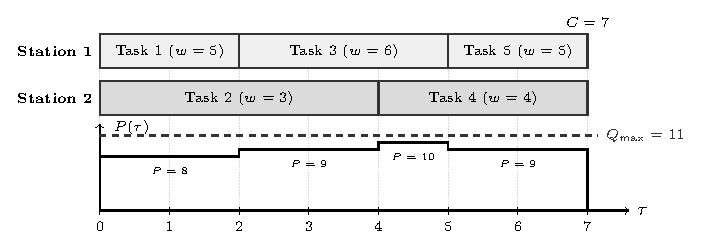
\includegraphics[width=0.85\textwidth]{figures/fig_example}
\caption{A feasible two-station schedule with cycle time $C=7$. Its line-power profile peaks at $10<\Qmax=11$.}
\label{fig:example}
\end{figure}

\section{Exact formulations and algorithms}
\label{sec:method}

\subsection{Fixed-horizon compact SAT encoding}

For a candidate cycle time $C$, let $H=\{0,\ldots,C-1\}$ and $H_i=\{0,\ldots,h_i\}$ with $h_i=C-t_i$. Variables $X_{i,k}$, $S_{i,s}$, and $A_{i,\tau}$ have the meanings in Table~\ref{tab:notation}. The cumulative variables are
\[
R_{i,k}\equiv\bigvee_{\ell=1}^{k}X_{i,\ell}\quad(k<m),
\qquad
T_{i,u}\equiv\bigvee_{s=0}^{u}S_{i,s}\quad(u<h_i).
\]
They adapt the compact SAT encoding (CSE) for SALB3PM \citep{VanKieu2025Compact}, based on sequential cardinality ideas \citep{sinz_sequential}, to the fixed peak power constraint studied here.

For $m\geq2$, exactly one station is selected by
\begin{alignat}{2}
R_{i,1}&\Leftrightarrow X_{i,1}, && i\in N, \tag{CSE-1}\\
R_{i,k-1}&\Rightarrow R_{i,k}, && k=2,\ldots,m-1, \tag{CSE-2}\\
X_{i,k}&\Rightarrow R_{i,k}, && k=2,\ldots,m-1, \tag{CSE-3}\\
X_{i,k}&\Rightarrow\neg R_{i,k-1}, && k=2,\ldots,m-1, \tag{CSE-4}\\
R_{i,k}\wedge\neg R_{i,k-1}&\Rightarrow X_{i,k}, && k=2,\ldots,m-1, \tag{CSE-5}\\
X_{i,m}&\Leftrightarrow\neg R_{i,m-1}. && \tag{CSE-5a}
\end{alignat}
For $m=1$, $X_{i,1}$ is a unit clause. Station-order precedence is
\begin{equation}
X_{i,k+1}\Rightarrow\neg R_{j,k}
\qquad (i,j)\in E,\ k=1,\ldots,m-1.
\tag{CSE-6}
\label{eq:cse6}
\end{equation}

If $h_i\geq1$, exactly one start is encoded by
\begin{alignat}{2}
T_{i,0}&\Leftrightarrow S_{i,0}, && \tag{CSE-7}\\
T_{i,u-1}&\Rightarrow T_{i,u}, && u=1,\ldots,h_i-1, \tag{CSE-8}\\
S_{i,u}&\Rightarrow T_{i,u}, && u=1,\ldots,h_i-1, \tag{CSE-9}\\
S_{i,u}&\Rightarrow\neg T_{i,u-1}, && u=1,\ldots,h_i-1, \tag{CSE-10}\\
T_{i,u}\wedge\neg T_{i,u-1}&\Rightarrow S_{i,u}, && u=1,\ldots,h_i-1, \tag{CSE-11}\\
S_{i,h_i}&\Leftrightarrow\neg T_{i,h_i-1}. && \tag{CSE-11a}
\end{alignat}
If $h_i=0$, the unit clause $S_{i,0}$ is used (CSE-11b).

To represent boundary cases uniformly, define the extended cumulative value
\begin{equation}
\widetilde T_{i,u}=\begin{cases}
\bot,&u<0,\\
T_{i,u},&0\leq u<h_i,\\
\top,&u\geq h_i.
\end{cases}
\label{eq:extended-t}
\end{equation}
Selected starts imply all actual activity slots,
\begin{equation}
S_{i,s}\Rightarrow A_{i,s+\ell}
\quad s\in H_i,\ \ell=0,\ldots,t_i-1,
\tag{CSE-12}
\label{eq:cse12}
\end{equation}
and same-station precedence is
\begin{equation}
X_{i,k}\wedge X_{j,k}\wedge S_{i,s}
\Rightarrow\neg\widetilde T_{j,s+t_i-1}
\quad (i,j)\in E,\ k\in K,\ s\in H_i.
\tag{CSE-13}
\label{eq:cse13}
\end{equation}
When $s+t_i-1\geq h_j$, avoiding overlap would require $\sigma_j\geq s+t_i>h_j$, which exceeds task $j$'s latest feasible start. The extended cumulative value is therefore true, and the clause correctly forbids the corresponding assignment\textendash{}start combination.

The baseline CSE activity-based non-overlap constraint \citep{VanKieu2025Compact} is
\begin{equation}
X_{i,k}\wedge X_{j,k}\wedge A_{i,\tau}\Rightarrow\neg A_{j,\tau}
\quad i<j,\ k\in K,\ \tau\in H.
\tag{CSE-14}
\label{eq:cse14}
\end{equation}
Classical station windows \citep{Scholl2006} use transitive predecessor and successor sets $P^*(i)$ and $S^*(i)$:
\begin{equation}
\mathrm{First}(i)=\left\lceil\frac{t_i+\sum_{h\in P^*(i)}t_h}{C}\right\rceil,
\quad
\mathrm{Last}(i)=m+1-\left\lceil\frac{t_i+\sum_{h\in S^*(i)}t_h}{C}\right\rceil.
\label{eq:first-last}
\end{equation}
Thus station-window pruning is expressed by
\begin{equation}
\neg X_{i,k}
\qquad k<\mathrm{First}(i)\ \text{or}\ k>\mathrm{Last}(i).
\tag{CSE-15}
\end{equation}
For every remaining pair $(i,k)$, a forward pass in topological order and a backward pass in reverse order compute valid bounds $e_{i,k}$ and $\ell_{i,k}$ on its start. The corresponding temporal pruning is
\begin{equation}
X_{i,k}\Rightarrow\neg S_{i,s}
\qquad s<e_{i,k}\ \text{or}\ s>\ell_{i,k}.
\tag{CSE-16}
\end{equation}
The passes apply the necessary completion-before-start relation whenever a precedence neighbor can occupy the same station. They only remove station--start choices that violate a derived precedence bound. A further optional strengthening is
\begin{equation}
A_{i,\tau}
\quad t_i\geq C/2,\quad \tau=C-t_i,\ldots,t_i-1
\tag{CSE-17}
\end{equation}
which forces the middle slots common to every placement of a long task. As elsewhere in the encoding, an equation consisting of a literal denotes a unit clause that forces that literal to true. These units are implied by CSE-12 and the exactly-one start block. CSE-17 is therefore optional and was disabled uniformly in the experiments reported here.

At each time slot, the pseudo-Boolean (PB) power constraint is
\begin{equation}
\sum_{i\in N}w_iA_{i,\tau}\leq\Qmax
\qquad \tau\in H.
\tag{PPC}
\label{eq:sat-power}
\end{equation}
Only the implication from a selected start to activity is needed for soundness: any extra true $A$ variables can only tighten \eqref{eq:sat-power}. Completeness follows by setting $A$ exactly to the activity of a feasible schedule.

The primary model instantiates CSE-6 and CSE-13 on the original edge set $E$. A separate configuration uses a sparse two-hop augmentation: tasks are processed in stored order with a persistent visited set, and for each unvisited root $i$, the preprocessing pass explores its reachable subgraph and inserts $(i,k)$ for each exposed two-edge path $i\to j\to k$. The resulting set is denoted $\Eaug$. Every added arc is implied by $E$, so the feasible schedules are unchanged; unlike a full transitive closure, the pass retains only a selected subset of redundant two-hop arcs. This configuration is evaluated separately and is not used as the default.

\subsection{Same-station encodings}
\label{sec:sm}

The Prior CSE configuration uses CSE-14 directly. The proposed SM and SM-T alternatives introduce $D_{i,j}$ for every $i<j$, meaning that the pair shares a station:
\begin{align}
X_{i,k}\wedge X_{j,k}&\Rightarrow D_{i,j}, && k\in K, \tag{SM-1}\\
X_{i,k}\wedge X_{j,\ell}&\Rightarrow\neg D_{i,j}, && k\neq\ell. \tag{SM-2}
\end{align}
The implementation enumerates every ordered choice $k\neq\ell$ in SM-2. SM prevents overlap with
\begin{equation}
D_{i,j}\wedge A_{i,\tau}\Rightarrow\neg A_{j,\tau}
\qquad i<j,\ \tau\in H.
\tag{SM-3}
\end{equation}
SM-T replaces SM-3 with the disjunction that task $j$ completes before $i$ starts or begins after $i$ completes:
\begin{equation}
\neg D_{i,j}\vee\neg S_{i,s}\vee
\widetilde T_{j,s-t_j}\vee
\neg\widetilde T_{j,s+t_i-1}
\qquad i<j,\ s\in H_i.
\tag{SM-T}
\label{eq:smt}
\end{equation}
Standard Boolean simplification handles constants from \eqref{eq:extended-t}: a true literal renders the clause a tautology and is omitted, while a false literal is removed. The name SM-T distinguishes this encoding from satisfiability modulo theories.

\subsection{Correctness and size}

\begin{lemma}
For each task, CSE-1--CSE-5a select exactly one workstation and satisfy $R_{i,k}=1$ if and only if the selected station is at most $k$. Similarly, CSE-7--CSE-11b select exactly one start time and satisfy $T_{i,u}=1$ if and only if the selected start is at most $u$.
\end{lemma}

\begin{proof}
For $m\geq2$, CSE-2 makes the $R$ chain monotone. If all entries are true, CSE-1 selects station~1; an interior false-to-true transition selects its unique station through CSE-3--CSE-5; and if all entries are false, CSE-5a selects station~$m$. The same clauses forbid every other $X_{i,k}$, while the unit clause covers $m=1$. The temporal chain is identical: CSE-7 and CSE-11a handle its two boundaries, CSE-8--CSE-11 handle a unique interior transition, and CSE-11b covers $h_i=0$. These cases also establish the stated prefix semantics of $R$ and $T$.
\end{proof}

\begin{lemma}
CSE-15--CSE-17 preserve every feasible schedule.
\end{lemma}

\begin{proof}
The workload of task $i$ and all its transitive predecessors requires at least $\mathrm{First}(i)$ stations up to and including $i$; applying the same argument to successors from the end of the line gives $\mathrm{Last}(i)$. The forward and backward passes propagate only necessary precedence completion bounds, so induction along the corresponding topological order proves $e_{i,k}\leq\sigma_i\leq\ell_{i,k}$ whenever task $i$ uses station $k$. Finally, every interval of length $t_i\geq C/2$ within $[0,C)$ contains the slots $C-t_i,\ldots,t_i-1$, which proves CSE-17.
\end{proof}

\begin{proposition}
For fixed $C$ and $\Qmax$, the formula consisting of CSE-1--CSE-13, one of the three non-overlap blocks, CSE-15--CSE-16, PPC, and optionally CSE-17 is satisfiable if and only if a feasible schedule with cycle time at most $C$ exists.
\end{proposition}

\begin{proof}
For soundness, take any satisfying assignment. The first lemma yields unique values $a(i)$ and $\sigma_i$. CSE-6 gives $a(i)\leq a(j)$ for every precedence arc. If $a(i)=a(j)$, CSE-13 and the extended-prefix semantics imply $\sigma_j\geq\sigma_i+t_i$; when the cutoff exceeds $j$'s latest start, the clause correctly forbids that station--start combination. The Prior CSE, SM, and SM-T configurations each exclude simultaneous activity of tasks sharing a station. In the latter two models, SM-1--SM-2 make $D_{i,j}$ true exactly for a same-station pair. CSE-12 makes every slot actually occupied by task $i$ true in $A_i$. Consequently, actual power is no greater than $\sum_iw_iA_{i,\tau}$, which PPC bounds by $\Qmax$. The second lemma shows that preprocessing removes no feasible choice. The induced schedule is therefore feasible.

For completeness, take a feasible schedule and set its selected $X$ and $S$ variables to true. Set $R$ and $T$ to their prefix meanings, set $A$ exactly on the occupied slots, and set $D_{i,j}$ according to station equality. Station order, temporal precedence, non-overlap, and PPC follow directly from feasibility. The two lemmas establish the cumulative and preprocessing blocks, so all clauses are satisfied.
\end{proof}

Table~\ref{tab:complexity} reports worst-case order while keeping the non-overlap term explicit. Here $\bar t$ is average processing time. PB auxiliary size depends on the selected encoder, coefficients, and threshold.

\begin{table}[t!]
\centering
\caption{Variable and constraint order of the structural encodings.}
\label{tab:complexity}
\small
\renewcommand{\arraystretch}{1.15}
\begin{tabularx}{\textwidth}{@{} Y c c @{}}
\toprule
Block & Variables & Clauses / PB constraints \\
\midrule
Assignment prefix & $O(nm)$ & $O(nm)$ \\
Start-time prefix & $O(nC)$ & $O(nC)$ \\
Station precedence & -- & $O(|E|m)$ \\
Same-station precedence & -- & $O(|E|mC)$ \\
Activity & $O(nC)$ & $O(nC\bar t)$ \\
Prior CSE non-overlap & -- & $O(n^2mC)$ \\
SM or SM-T & $O(n^2)$ & $O(n^2m^2+n^2C)$ \\
Station/start preprocessing & -- & $O(nm+n m C)$ \\
Peak power & encoder-dependent & $C$ PB constraints plus encoder clauses \\
\bottomrule
\end{tabularx}
\end{table}

For comparison, pairwise assignment and start-time at-most-one (AMO) constraints require $O(nm^2)$ and $O(nC^2)$ clauses, while pairwise precedence requires $O(|E|m^2)$ and $O(|E|mC^2)$. The prefix-variable encodings reduce these components to linear order in $m$ or $C$. The $O(n^2mC)$ non-overlap term remains in Prior CSE, and with $|E|=O(n^2)$ it determines that configuration's dominant structural order. Because SM-2 enumerates $k\neq\ell$, its station-sharing definition contributes $O(n^2m^2)$ clauses.

\subsection{Two-phase incremental SAT optimization}

For a model $\phi$ at horizon $H$, let
\begin{equation}
C(\phi)=\max\{s+t_i:S_{i,s}=1\}.
\end{equation}
A schedule better than incumbent $\Cbest$ must satisfy $\sigma_i+t_i\leq\Cbest-1$ for every task, represented by the unit literals
\begin{equation}
\Gamma(\Cbest)=\{T_{i,\Cbest-t_i-1}:i\in N\}.
\label{eq:cut}
\end{equation}
\begin{algorithm}[H]
\caption{Two-phase incremental SAT optimization}
\label{alg:incremental}
\begin{algorithmic}[1]
\Require Instance $(N,E,t,w,m,\Qmax)$ and Phase I conflict budget $B_F$
\Ensure Incumbent $\phi^*$, bounds $[LB,UB]$, and proof status
\If{$\Qmax<\max_i w_i$}
  \State \Return \Status{INFEASIBLE}
\EndIf
\State $LB\gets\LBzero$; $(\phi^*,UB)\gets\textsc{SequentialSchedule}()$
\State $H\gets\Cinit$; $H_{\mathrm{seq}}\gets UB$; $\mathit{ready}\gets\mathrm{false}$
\While{$H<H_{\mathrm{seq}}$} \Comment{Phase I: feasible-solution search}
  \State $(r,\phi,\mathcal S)\gets\textsc{SolveLimited}(\Phi(H,\Qmax),B_F)$
  \If{$r=\Status{SAT}$}
    \State $(\phi^*,UB)\gets(\phi,C(\phi))$; $\mathit{ready}\gets\mathrm{true}$; \textbf{break}
  \ElsIf{$r=\Status{UNSAT}$}
    \State $LB\gets\max\{LB,H+1\}$
  \EndIf \Comment{\Status{UNKNOWN} changes neither bound}
  \State $H\gets\min\{H_{\mathrm{seq}},\max(H+1,\lceil1.5H\rceil)\}$
\EndWhile
\If{$\neg\mathit{ready}$}
  \State $H\gets H_{\mathrm{seq}}$; $\mathcal S\gets\textsc{BuildSolver}(\Phi(H,\Qmax))$
  \State $(r,\phi)\gets\textsc{Solve}(\mathcal S)$
  \If{$r=\Status{TIMEOUT}$} \State \Return $(\phi^*,LB,UB,\Status{TIMEOUT})$ \EndIf
  \State $(\phi^*,UB)\gets(\phi,C(\phi))$
\EndIf
\While{$LB<UB$} \Comment{Phase II: incumbent improvement and proof}
  \If{some literal in $\Gamma(UB)$ has a negative index}
    \State $LB\gets UB$; \textbf{break}
  \EndIf
  \State add every literal in $\Gamma(UB)$ to $\mathcal S$
  \State $(r,\phi)\gets\textsc{SolveIncrementally}(\mathcal S)$
  \If{$r=\Status{UNSAT}$} \State $LB\gets UB$; \textbf{break} \EndIf
  \If{$r=\Status{TIMEOUT}$} \State \Return $(\phi^*,LB,UB,\Status{TIMEOUT})$ \EndIf
  \State $(\phi^*,UB)\gets(\phi,C(\phi))$
\EndWhile
\State \Return $(\phi^*,UB,UB,\Status{OPTIMAL})$
\end{algorithmic}
\end{algorithm}

Algorithm~\ref{alg:incremental} maintains the incumbent value as $UB$, so $\Gamma(UB)$ is \eqref{eq:cut} at the current incumbent. If any index in \eqref{eq:cut} is negative, no better cycle can contain that task and the incumbent is already optimal. Otherwise all required cumulative variables are defined within the current solver horizon.

Phase I separates the search for an improved feasible solution from the proof that a small candidate cycle time is infeasible. A conflict-limited call returning \Status{UNKNOWN} leaves $LB$ unchanged and the search advances to the next horizon, whereas a completed \Status{UNSAT} at $H$ raises the bound to $H+1$. The fixed expansion ratio of 1.5 reaches $C^{\mathrm{seq}}$ after a logarithmic number of model reconstructions. A \Status{SAT} result yields both an incumbent and a solver whose learned clauses are retained in Phase II. If Phase I finds no feasible solution, the sequential incumbent remains available and a solver is initialized at $C^{\mathrm{seq}}$. Until that call or another complete \Status{UNSAT} strengthens the bound, $LB$ remains $\LBzero$ or the largest previously certified infeasible horizon plus one.

The half-open activity convention explains the $-1$ in \eqref{eq:cut}: $T_{i,u}$ means $\sigma_i\leq u$, so completion by $UB-1$ requires $u=UB-t_i-1$. Each \Status{SAT} call made under the cut in \eqref{eq:cut} supplies a strictly smaller incumbent. \Status{UNSAT} under this cut excludes every schedule with cycle time below the incumbent, closes the interval $[LB,UB]$, and certifies optimality. A timeout returns both the validated incumbent and the strongest analytical or SAT-certified lower bound accumulated so far.

\begin{proposition}
Algorithm~\ref{alg:incremental} returns a feasible incumbent whenever $\Qmax\geq\max_i w_i$. If it returns \Status{OPTIMAL}, the reported cycle time is globally optimal.
\end{proposition}

\begin{proof}
The topological sequential schedule is feasible because it respects every precedence arc, has no station overlap, and activates at most one task, whose demand is at most $\Qmax$. Consequently, the formula at $H_{\mathrm{seq}}=C^{\mathrm{seq}}$ is satisfiable, so the \textsc{Solve} call in the $\neg\mathit{ready}$ branch cannot return \Status{UNSAT}, and the update $(\phi^*,UB)\gets(\phi,C(\phi))$ is always well-defined. Bounded \Status{UNKNOWN} calls do not alter either bound. Every update $LB\gets H+1$ follows only from a complete \Status{UNSAT} proof for all schedules of cycle time at most $H$. In Phase II, \eqref{eq:cut} represents all schedules strictly better than the incumbent within the fixed horizon. Therefore \Status{SAT} preserves feasibility while decreasing $UB$, and \Status{UNSAT} proves that no value below $UB$ exists. At termination with $LB=UB$, that common value is optimal.
\end{proof}

\subsection{Mathematical-programming formulations}

The mathematical-programming formulations use a valid upper modeling horizon $\bar C$; the sequential schedule supplies $\bar C=\sum_i t_i$ if no tighter valid horizon is available. Let $\bar H=\{0,\ldots,\bar C-1\}$ and $\bar H_i=\{0,\ldots,\bar C-t_i\}$. Binary variables $x_{i,k}$ and $y_{i,s}$ select a station and a start $s\in\bar H_i$, respectively. Define the linear activity expression
\begin{equation}
b_{i,\tau}=\sum_{s=\max\{0,\tau-t_i+1\}}^{\min\{\tau,\bar C-t_i\}}y_{i,s}.
\label{eq:mip-activity}
\end{equation}
Exactly one station and one start are selected:
\begin{equation}
\sum_{k\in K}x_{i,k}=1,
\qquad
\sum_{s\in\bar H_i}y_{i,s}=1
\qquad i\in N.
\label{eq:mip-one}
\end{equation}
For every $(i,j)\in E$ and $k\in K$, station order and same-station temporal order are imposed by
\begin{align}
x_{j,k}&\leq\sum_{h=1}^{k}x_{i,h}, \label{eq:mip-station-prec}\\
y_{j,s}&\leq\sum_{r=0}^{s-t_i}y_{i,r}+2-x_{i,k}-x_{j,k}
&&s\in\bar H_j, \label{eq:mip-time-prec}
\end{align}
where an empty sum is zero. Pairwise station capacity and the peak power constraint are
\begin{align}
x_{i,k}+x_{j,k}+b_{i,\tau}+b_{j,\tau}&\leq3
&&i<j,\ k\in K,\ \tau\in\bar H, \label{eq:mip-nonoverlap}\\
\sum_{i\in N}w_i b_{i,\tau}&\leq\Qmax
&&\tau\in\bar H. \label{eq:mip-power}
\end{align}
Finally, the integer objective variable $Z$ satisfies
\begin{align}
Z&\geq\sum_{s\in\bar H_i}s y_{i,s}+t_i &&i\in N, \label{eq:mip-z}\\
Z&\geq\sum_{i\in N}t_i x_{i,k} &&k\in K, \label{eq:mip-workload}
\end{align}
and the objective is $\min Z$. Constraint~\eqref{eq:mip-workload} is a valid workload strengthening. The time-indexed structure is employed because it expresses both instantaneous power and within-station non-overlap directly. Gurobi-MIP and CPLEX-MIP solve this formulation; CPLEX-CP uses the same logical model through the CP Optimizer backend.

\section{Experimental design}
\label{sec:experiment}

\subsection{Benchmark set, peak power thresholds, and SAT encodings}

The benchmark set comprises 72 cases formed by pairing 13 classical SALBP precedence graphs with prescribed station counts. Table~\ref{tab:benchmark-inventory} gives graph sizes and workstation ranges. Processing times and precedence relations are taken from the standard instance files. Each graph is augmented with a fixed vector of integer task power demands in $[5,50]$, applied consistently across all station counts, power thresholds, and solvers. Performance is summarized using both case-weighted and graph-balanced aggregate metrics.

\begin{table}[t!]
\centering
\caption{Benchmark set. Each case combines a precedence graph with a prescribed number of workstations $m$.}
\label{tab:benchmark-inventory}
\footnotesize
\renewcommand{\arraystretch}{1.15}
\setlength{\tabcolsep}{6pt}
\begin{tabular}{@{} l c c c c @{\quad} l c c c c @{}}
\toprule
Graph & $n$ & Cases & $m_{\min}$ & $m_{\max}$ & Graph & $n$ & Cases & $m_{\min}$ & $m_{\max}$ \\
\midrule
BOWMAN & 8 & 1 & 5 & 5 & MANSOOR & 11 & 3 & 2 & 4 \\
BUXEY & 29 & 6 & 7 & 13 & MERTENS & 7 & 4 & 2 & 6 \\
GUNTHER & 35 & 6 & 7 & 14 & MITCHELL & 21 & 3 & 3 & 8 \\
HESKIA & 28 & 4 & 3 & 8 & ROSZIEG & 25 & 4 & 4 & 10 \\
JACKSON & 11 & 5 & 3 & 8 & SAWYER & 30 & 8 & 5 & 14 \\
JAESCHKE & 9 & 4 & 3 & 8 & WARNECKE & 58 & 13 & 14 & 31 \\
LUTZ2 & 89 & 11 & 24 & 49 &  &  &  &  &  \\
\addlinespace[3pt]
\multicolumn{10}{@{}c}{\textit{Total: \MainFamilyCount{} precedence graphs and \MainInstanceCount{} benchmark cases}} \\
\bottomrule
\end{tabular}
\end{table}

\begin{table}[t!]
\centering
\caption{Certification source of the uncapped SALBP-2 reference optima.}
\label{tab:no-peak-reference}
\footnotesize
\renewcommand{\arraystretch}{1.15}
\setlength{\tabcolsep}{5pt}
\begin{threeparttable}
\begin{tabular}{@{} l c l @{}}
\toprule
Reference source & Cases & Certification role \\
\midrule
Scholl SALBP-2 benchmark ($c^*$) & 35 & Published exact SALBP-2 optimum \\
Scholl SALBP-1 feasible $c$ + No-Peak SAT & 35 & SAT reports optimality \\
Scholl SALBP-1 feasible $c$ + workload LB & 2 & $\lceil\sum_i t_i/m\rceil = c$ \\
\bottomrule
\end{tabular}
\begin{tablenotes}[flushleft]
\scriptsize
\item The SALBP-1 column is a feasible upper bound for SALBP-2, not an optimum certificate by itself. Benchmark values are from \citet{SchollBenchmark1993}.
\end{tablenotes}
\end{threeparttable}
\end{table}

The experiments vary three factors: the peak power limit ($Q_{\max}^{\mathrm{top}}$ or $Q_{\max}^{\mathrm{avg}}$), the cycle-time search strategy (Direct or Two-phase), and the non-overlap encoding (Prior CSE, SM, or SM-T). Both search strategies are tested on the original edge set $E$; the sparse augmentation $E^+$ is evaluated separately under Direct search only. Prior CSE denotes the compact CSE-14 non-overlap encoding \citep{VanKieu2025Compact} and serves as the baseline formulation. Table~\ref{tab:sat-configurations} lists all tested configurations.

\begin{table}[t!]
\centering
\caption{Evaluated SAT configurations.}
\label{tab:sat-configurations}
\footnotesize
\renewcommand{\arraystretch}{1.15}
\setlength{\tabcolsep}{14pt}
\begin{threeparttable}
\begin{tabular}{@{} l c c l @{}}
\toprule
ID & Search strategy & Arcs & Non-overlap block \\
\midrule
D-CSE/$E$ & Direct & $E$ & Prior CSE (CSE-14) \\
D-SM/$E$ & Direct & $E$ & SM (SM-1--SM-3) \\
D-SM-T/$E$ & Direct & $E$ & SM-T (SM-1--SM-2, SM-T) \\
\addlinespace[2pt]
2P-CSE/$E$ & Two-phase & $E$ & Prior CSE (CSE-14) \\
2P-SM/$E$ & Two-phase & $E$ & SM (SM-1--SM-3) \\
2P-SM-T/$E$ & Two-phase & $E$ & SM-T (SM-1--SM-2, SM-T) \\
\addlinespace[2pt]
D-CSE/$E^+$ & Direct & $E^+$ & Prior CSE (CSE-14) \\
D-SM/$E^+$ & Direct & $E^+$ & SM (SM-1--SM-3) \\
D-SM-T/$E^+$ & Direct & $E^+$ & SM-T (SM-1--SM-2, SM-T) \\
\bottomrule
\end{tabular}
\begin{tablenotes}[flushleft]
\scriptsize
\item Prior CSE is the baseline CSE-14 activity-based non-overlap block \citep{VanKieu2025Compact}. Every configuration is evaluated under both $Q^{\mathrm{top}}_{\max}$ and $Q^{\mathrm{avg}}_{\max}$ on all 72 benchmark cases. Two-phase search is evaluated on $E$.
\end{tablenotes}
\end{threeparttable}
\end{table}

Every benchmark case is evaluated under both thresholds in \eqref{eq:q-top}--\eqref{eq:q-avg}; $Q_{\max}^{\mathrm{avg}}<Q_{\max}^{\mathrm{top}}$ holds in all 72 cases. The main experimental matrix combines Direct and Two-phase search, three non-overlap encodings on $E$, two power limits, and 72 cases, yielding 864 runs. A separate set of 432 Direct runs tests the same encodings on $E^+$ under both limits. Direct search begins exact optimization at $\Cinit$, whereas Two-phase search first applies the conflict-limited feasibility checks of Algorithm~\ref{alg:incremental}. All reported clause counts omit CSE-17. Threshold comparisons report both $\alpha_Q$ and $s_Q$ because the average-based and top-$m$-based constructions occupy different regions of the normalized tightness scale.

\FloatBarrier
\subsection{Computational protocol and solver scope}

All experiments were conducted on Google Cloud Platform c4-highcpu-8 instances (8 vCPUs, 16 GB RAM, Ubuntu 20.04 LTS) with a 3,600-second wall-clock limit per run; reported times include model construction and all solver calls. The SAT solver was CaDiCaL 1.9.5 accessed via PySAT, with Binary Merger encoding for pseudo-Boolean constraints \citep{Ignatiev2018PySAT,Biere2024CaDiCaL}. The commercial comparators were Gurobi-MIP, CPLEX-MIP, and CPLEX-CP (CPLEX 22.1.1). CaDiCaL ran on a single thread; the commercial solvers used their default multi-thread settings on the same machine. Gurobi applied a 4 GB soft memory limit. Wall-clock comparisons therefore reflect deployment-level differences rather than equal-core algorithmic ratios. Every reported schedule was independently validated against task assignment, precedence, within-station non-overlap, cycle-time, and peak-power feasibility.

The Two-phase search uses the analytical bound in \eqref{eq:cycle-lb} as its initial lower bound, the sequential schedule as an immediately available incumbent, and a fixed conflict budget of $B_F=50{,}000$ per Phase-I probe. These parameters are implementation constants applied uniformly across all graphs, station counts, and power limits; no instance-specific tuning is performed. Direct search omits Phase I and begins exact optimization at $\Cinit$. Both strategies operate under the same 3,600-second time limit.

\subsection{Reference values and performance measures}

A run is counted as solved to optimality only when the solver reports \Status{OPTIMAL}; a feasible objective value reported at timeout remains an incumbent and an upper bound. For each case and threshold, the best-known solution (BKS), denoted $C^{\mathrm{BKS}}$, is the smallest incumbent across all methods. It is labeled OPT when at least one method certifies that value and UB otherwise. The relative percentage deviation (RPD) of solver $s$ from the BKS is
\begin{equation}
\operatorname{RPD}_{\mathrm{BKS}}(s)=
100\frac{UB_s-C^{\mathrm{BKS}}}{C^{\mathrm{BKS}}}.
\label{eq:rpd-bks}
\end{equation}
When a run supplies both bounds, its certified relative gap is
\begin{equation}
\operatorname{Gap}_{\mathrm{cert}}(s)=
100\frac{UB_s-LB_s}{UB_s}.
\label{eq:cert-gap}
\end{equation}
Mean RPD is computed over runs with an incumbent; PAR-2 and proof counts cover all 72 cases. PAR-2 assigns the observed runtime to proven-optimal runs and twice the time limit (7,200~s) to all other runs; it measures proof completion but does not distinguish feasible-but-unproven outcomes from runs without an incumbent, a limitation addressed jointly by the BKS and RPD metrics. Proof times for \Status{OPTIMAL} runs are summarized by method-wise medians and geometric means; paired geometric-mean ratios are restricted to cases in which both compared methods certify the same optimum. Cactus plots show cumulative proven-optimal counts against wall-clock time.

All \NoPeakOptCount{} uncapped SALBP-2 reference optima are exact: \NoPeakSATProvenCount{} are proved optimal by SAT within the time limit, and the remaining \NoPeakExternalOnlyCount{} match published exact SALBP-2 benchmark values \citep{SchollBenchmark1993} or analytical workload lower bounds. A reported cycle time difference $\Delta C$ represents the increase relative to this certified uncapped optimum.

\subsection{Research questions}

The experiments address four research questions. RQ1 measures how each power threshold changes the best-known cycle time relative to the uncapped optimum and how the change varies with normalized threshold tightness $s_Q$. RQ2 compares Direct and Two-phase search, both initialized at $\Cinit$, on BKS values, proven optima, mean RPD, PAR-2, and paired wall time. RQ3 compares the Prior CSE, SM, and SM-T encodings in formula size and runtime; the effect of $E^+$ is evaluated separately under Direct search. RQ4 compares the selected SAT configurations with Gurobi-MIP, CPLEX-MIP, and CPLEX-CP on feasible-solution coverage, BKS values, proven optima, mean RPD, PAR-2, and wall time.

For RQ4, one SAT configuration is selected per power limit by the same pre-specified lexicographic rule: maximize proven optima, then minimize PAR-2, then maximize BKS hits, then minimize mean RPD. The rule is applied to the six Direct/Two-phase configurations on $E$; Table~\ref{tab:sat-main-results} reports all six to make the selection transparent.

The hardness analysis in Section~\ref{sec:results} groups the 72 cases by tasks per station $n/m$, direct precedence density, and the normalized energy lower-bound ratio $\rho_E=\lceil\sum_iw_it_i/\Qmax\rceil/C^{\mathrm{BKS}}_0$, where $C^{\mathrm{BKS}}_0$ is the uncapped optimum.

\section{Results and discussion}
\label{sec:results}



\subsection{RQ1: power-limit tightness and cycle time increase}

Table~\ref{tab:cap-impact} compares the BKS under each power limit with the uncapped optimum. Under $Q_{\max}^{\mathrm{top}}$, all 72 cases have a BKS: six equal the uncapped optimum and 66 exceed it, with a mean difference of 16.49\% and median 14.29\%. Under $Q_{\max}^{\mathrm{avg}}$, all 72 BKS values exceed the uncapped optimum, with mean 60.99\% and median 62.20\%. The normalized position of $Q_{\max}^{\mathrm{top}}$ occupies a narrow band, $\alpha_Q=\AlphaQTopMin$--$\AlphaQTopMax$, because the construction $\alpha_Q=\lfloor d/2\rfloor/d$ takes only two values for odd and even $d=UB_Q-LB_Q$. The average-based construction spans $\alpha_Q=\AlphaQAVGMin$--$\AlphaQAVGMax$ (median $\AlphaQAVGMedian$) and is tighter than $Q_{\max}^{\mathrm{top}}$ in every case.

\begin{table}[t!]
\centering
\caption{Best-known cycle time increase under each peak power threshold relative to the independently certified uncapped SALBP-2 optimum.}
\label{tab:cap-impact}
\footnotesize
\renewcommand{\arraystretch}{1.15}
\setlength{\tabcolsep}{3.5pt}
\begin{threeparttable}
\begin{tabular*}{\textwidth}{@{\extracolsep{\fill}} l c c c c c c c @{}}
\toprule
Threshold & Feasible BKS & BKS proven & Same $C$ & Higher $C$ & Mean $\Delta C$ & Mean $\Delta C$ (\%) & Median $\Delta C$ (\%) \\
\midrule
$Q^{\mathrm{top}}_{\max}$ & 72 & 45 & 6 & 66 & 7.07 & 16.49\% & 14.29\% \\
$Q^{\mathrm{avg}}_{\max}$ & 72 & 25 & 0 & 72 & 30.32 & 60.99\% & 62.20\% \\
\bottomrule
\end{tabular*}
\begin{tablenotes}[flushleft]
\scriptsize
\item Feasible BKS counts cases with a feasible solution. BKS proven counts cases certified optimal by at least one solver. The uncapped reference values are exact optima from the SALBP-2 benchmark literature and No-Peak SAT proofs; $\Delta C$ measures the increase relative to these reference optima.
\end{tablenotes}
\end{threeparttable}
\end{table}

The BKS under $Q_{\max}^{\mathrm{avg}}$ exceeds that under $Q_{\max}^{\mathrm{top}}$ in 68 cases and equals it in four; it is never smaller. Figure~\ref{fig:cap-effect}(a) shows this comparison. Panel~(b) shows that the top-$m$ construction occupies $s_Q=\TightnessTopMin$--$\TightnessTopMax$, whereas the average-based construction spans $\TightnessAVGMin$--$\TightnessAVGMax$; the BKS increase varies within this wider range, so $s_Q$ alone does not explain the cycle time change. The BKS is proven optimal for 45 cases under $Q_{\max}^{\mathrm{top}}$ and 25 under $Q_{\max}^{\mathrm{avg}}$ (by at least one of the tested SAT configurations); the remaining entries are valid feasible upper bounds. Graph-balanced weighting gives mean increases of \GraphBalancedTopPenaltyPct\% and \GraphBalancedAVGPenaltyPct\%, confirming that the average-based cap produces the larger increase regardless of the weighting scheme.

\begin{figure}[H]
\centering
\begin{minipage}{0.49\textwidth}
\centering
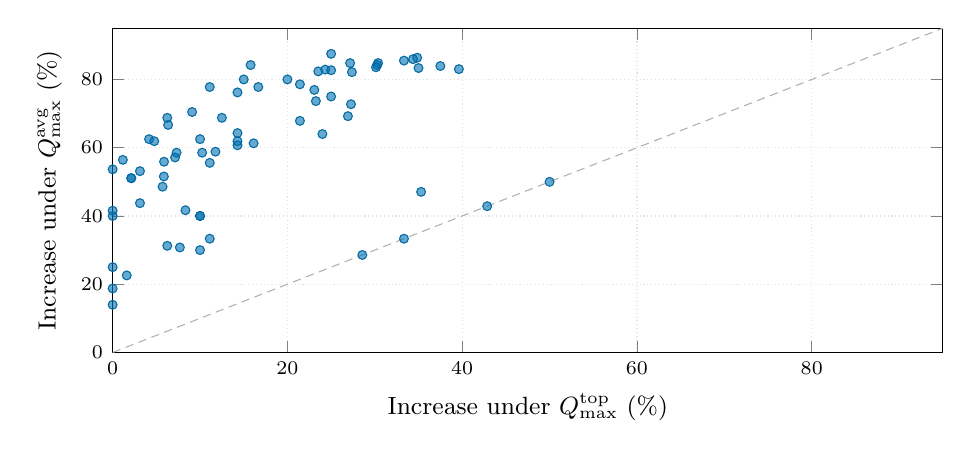
\begin{tikzpicture}
\begin{axis}[width=\linewidth,height=57mm,xmin=0,xmax=95,ymin=0,ymax=95,xtick={0,20,40,60,80},ytick={0,20,40,60,80},xlabel={Increase under $Q^{\mathrm{top}}_{\max}$ (\%)},ylabel={Increase under $Q^{\mathrm{avg}}_{\max}$ (\%)},grid=major,grid style={gray!22,densely dotted},tick label style={font=\scriptsize},label style={font=\small}]
\addplot[domain=0:95,samples=2,no marks,gray!60,densely dashed] {x};
\addplot[only marks,mark=*,mark size=1.6pt,mark options={draw=PlotBlue!90!black,fill=PlotBlue,fill opacity=0.6,draw opacity=0.95}] coordinates {(35.294118,47.058824) (5.882353,55.882353) (3.125000,53.125000) (14.285714,60.714286) (11.111111,55.555556) (2.127660,51.063830) (0.000000,53.658537) (6.250000,68.750000) (9.090909,70.454545) (10.000000,62.500000) (4.166667,62.500000) (6.349206,66.666667) (11.111111,77.777778) (1.169591,56.432749) (5.859375,51.562500) (10.243902,58.536585) (23.255814,73.643411) (6.250000,31.250000) (8.333333,41.666667) (10.000000,40.000000) (11.111111,33.333333) (42.857143,42.857143) (7.692308,30.769231) (10.000000,30.000000) (0.000000,25.000000) (33.333333,33.333333) (14.285714,76.190476) (15.000000,80.000000) (15.789474,84.210526) (16.666667,77.777778) (23.529412,82.352941) (25.000000,87.500000) (20.000000,80.000000) (21.428571,78.571429) (23.076923,76.923077) (25.000000,75.000000) (27.272727,72.727273) (0.000000,13.978495) (1.612903,22.580645) (0.000000,18.750000) (0.000000,40.000000) (10.000000,40.000000) (28.571429,28.571429) (50.000000,50.000000) (5.714286,48.571429) (14.285714,61.904762) (14.285714,64.285714) (7.142857,57.142857) (3.125000,43.750000) (4.761905,61.904762) (12.500000,68.750000) (11.764706,58.823529) (16.129032,61.290323) (21.428571,67.857143) (26.923077,69.230769) (24.000000,64.000000) (0.000000,41.538462) (2.127660,51.063830) (7.317073,58.536585) (24.324324,82.882883) (25.000000,82.692308) (27.173913,84.782609) (27.380952,82.142857) (30.379747,84.810127) (30.263158,84.210526) (30.136986,83.561644) (33.333333,85.507246) (34.848485,86.363636) (34.375000,85.937500) (35.000000,83.333333) (37.500000,83.928571) (39.622642,83.018868)};
\end{axis}
\end{tikzpicture}
\par\smallskip\footnotesize (a) Within-case comparison
\end{minipage}
\hfill
\begin{minipage}{0.49\textwidth}
\centering
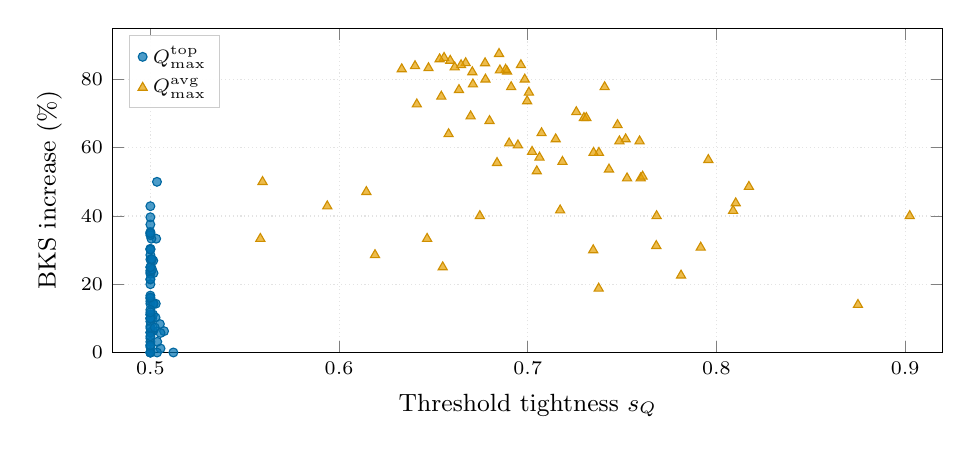
\begin{tikzpicture}
\begin{axis}[width=\linewidth,height=57mm,xmin=0.48,xmax=0.92,ymin=0,ymax=95,xtick={0.5,0.6,0.7,0.8,0.9},ytick={0,20,40,60,80},xlabel={Threshold tightness $s_Q$},ylabel={BKS increase (\%)},yticklabel style={font=\scriptsize},xticklabel style={font=\scriptsize},label style={font=\small},grid=major,grid style={gray!22,densely dotted},legend style={font=\scriptsize,at={(0.02,0.98)},anchor=north west,draw=gray!40,fill=white,fill opacity=0.95}]
\addplot[only marks,mark=*,mark size=1.6pt,mark options={draw=PlotBlue!90!black,fill=PlotBlue,fill opacity=0.7}] coordinates {(0.500000,35.294118) (0.500000,5.882353) (0.500000,3.125000) (0.501241,14.285714) (0.500000,11.111111) (0.500000,2.127660) (0.500000,0.000000) (0.501155,6.250000) (0.500000,9.090909) (0.500914,10.000000) (0.500000,4.166667) (0.501618,6.349206) (0.501425,11.111111) (0.505376,1.169591) (0.500000,5.859375) (0.502732,10.243902) (0.501650,23.255814) (0.507246,6.250000) (0.505051,8.333333) (0.500000,10.000000) (0.500000,11.111111) (0.500000,42.857143) (0.500000,7.692308) (0.500000,10.000000) (0.500000,0.000000) (0.503067,33.333333) (0.500000,14.285714) (0.500000,15.000000) (0.500000,15.789474) (0.500000,16.666667) (0.500000,23.529412) (0.500412,25.000000) (0.500000,20.000000) (0.500000,21.428571) (0.500000,23.076923) (0.500000,25.000000) (0.500000,27.272727) (0.500000,0.000000) (0.500000,1.612903) (0.503546,0.000000) (0.512195,0.000000) (0.500000,10.000000) (0.500000,28.571429) (0.503497,50.000000) (0.505376,5.714286) (0.502857,14.285714) (0.501742,14.285714) (0.500000,7.142857) (0.503650,3.125000) (0.500000,4.761905) (0.500000,12.500000) (0.500000,11.764706) (0.500000,16.129032) (0.500000,21.428571) (0.501529,26.923077) (0.500000,24.000000) (0.500000,0.000000) (0.500000,2.127660) (0.502326,7.317073) (0.500876,24.324324) (0.500000,25.000000) (0.500730,27.173913) (0.500659,27.380952) (0.500000,30.379747) (0.500000,30.263158) (0.500000,30.136986) (0.500554,33.333333) (0.500000,34.848485) (0.500000,34.375000) (0.500000,35.000000) (0.500000,37.500000) (0.500000,39.622642)};
\addlegendentry{$Q^{\mathrm{top}}_{\max}$}
\addplot[only marks,mark=triangle*,mark size=1.9pt,mark options={draw=PlotOrange!90!black,fill=PlotOrange,fill opacity=0.7}] coordinates {(0.614458,47.058824) (0.718391,55.882353) (0.704787,53.125000) (0.694789,60.714286) (0.683721,55.555556) (0.759843,51.063830) (0.743056,53.658537) (0.729792,68.750000) (0.725738,70.454545) (0.714808,62.500000) (0.751880,62.500000) (0.747573,66.666667) (0.740741,77.777778) (0.795699,56.432749) (0.760870,51.562500) (0.737705,58.536585) (0.699670,73.643411) (0.768116,31.250000) (0.717172,41.666667) (0.674603,40.000000) (0.646667,33.333333) (0.593750,42.857143) (0.791667,30.769231) (0.734694,30.000000) (0.654930,25.000000) (0.558282,33.333333) (0.700617,76.190476) (0.698413,80.000000) (0.696360,84.210526) (0.691203,77.777778) (0.689024,82.352941) (0.684774,87.500000) (0.677591,80.000000) (0.670940,78.571429) (0.663539,76.923077) (0.654182,75.000000) (0.641204,72.727273) (0.875000,13.978495) (0.781250,22.580645) (0.737589,18.750000) (0.902439,40.000000) (0.768293,40.000000) (0.619048,28.571429) (0.559441,50.000000) (0.817204,48.571429) (0.748571,61.904762) (0.707317,64.285714) (0.706215,57.142857) (0.810219,43.750000) (0.759259,61.904762) (0.731034,68.750000) (0.702290,58.823529) (0.690141,61.290323) (0.679739,67.857143) (0.669725,69.230769) (0.658046,64.000000) (0.808824,41.538462) (0.752632,51.063830) (0.734884,58.536585) (0.688266,82.882883) (0.685246,82.692308) (0.677372,84.782609) (0.670619,82.142857) (0.667085,84.810127) (0.664663,84.210526) (0.661290,83.561644) (0.658915,85.507246) (0.655650,86.363636) (0.653292,85.937500) (0.647399,83.333333) (0.640255,83.928571) (0.633218,83.018868)};
\addlegendentry{$Q^{\mathrm{avg}}_{\max}$}
\end{axis}
\end{tikzpicture}
\par\smallskip\footnotesize (b) Relative increase versus $s_Q$
\end{minipage}
\caption{Best-known cycle time increases under the two peak power threshold constructions. Panel~(a) compares the 72 benchmark cases with a feasible BKS under both thresholds; the dashed line denotes equality. Panel~(b) shows all 144 benchmark-case/threshold records.}
\label{fig:cap-effect}
\end{figure}

\FloatBarrier
\subsection{RQ2: Direct versus Two-phase search from $\Cinit$}

Table~\ref{tab:sat-main-results} reports the six combinations of search strategy and encoding; every combination finds a feasible solution for all 72 cases. Under $Q_{\max}^{\mathrm{top}}$, D-SM/$E$ and 2P-SM-T/$E$ each find 71 BKS values with mean RPD 0.01\%. Three configurations tie at 44 proven optima (D-CSE/$E$, D-SM/$E$, and D-SM-T/$E$); D-SM/$E$ attains the lowest PAR-2, 2911.2 seconds, consistent with the lexicographic selection rule in Section~\ref{sec:experiment}, so it is selected for the solver comparison.

\begin{table}[t!]
\centering
\caption{End-of-run performance of all six Direct and Two-phase SAT configurations on $E$.}
\label{tab:sat-main-results}
\footnotesize
\renewcommand{\arraystretch}{1.15}
\setlength{\tabcolsep}{5pt}
\begin{threeparttable}
\begin{tabular}{@{} l c c c c @{}}
\toprule
Configuration & BKS & Proven & Mean RPD & PAR-2 (s) \\
\midrule
\multicolumn{5}{@{}l}{\textit{Top-$m$-based threshold ($Q^{\mathrm{top}}_{\max}$)}} \\
\addlinespace[2pt]
D-CSE/$E$ & 70 / 72 & \textbf{44 / 72} & 0.02\% & 2919.2 \\
2P-CSE/$E$ & 69 / 72 & \textbf{44 / 72} & 0.09\% & 2933.5 \\
\addlinespace[1pt]
D-SM/$E$ & \textbf{71 / 72} & \textbf{44 / 72} & \textbf{0.01\%} & \textbf{2911.2} \\
2P-SM/$E$ & 70 / 72 & 43 / 72 & 0.02\% & 2965.5 \\
\addlinespace[1pt]
D-SM-T/$E$ & 70 / 72 & \textbf{44 / 72} & 0.08\% & 2918.7 \\
2P-SM-T/$E$ & \textbf{71 / 72} & 43 / 72 & \textbf{0.01\%} & 2988.5 \\
\addlinespace[4pt]
\multicolumn{5}{@{}l}{\textit{Average-based threshold ($Q^{\mathrm{avg}}_{\max}$)}} \\
\addlinespace[2pt]
D-CSE/$E$ & 62 / 72 & 22 / 72 & 0.25\% & 5008.4 \\
2P-CSE/$E$ & 61 / 72 & 23 / 72 & 0.20\% & 4957.7 \\
\addlinespace[1pt]
D-SM/$E$ & \textbf{64 / 72} & 23 / 72 & 0.18\% & 4954.6 \\
2P-SM/$E$ & 62 / 72 & 23 / 72 & 0.14\% & 4956.9 \\
\addlinespace[1pt]
D-SM-T/$E$ & 62 / 72 & 23 / 72 & 0.25\% & 4951.5 \\
2P-SM-T/$E$ & \textbf{64 / 72} & \textbf{24 / 72} & \textbf{0.11\%} & \textbf{4903.1} \\
\bottomrule
\end{tabular}
\begin{tablenotes}[flushleft]
\scriptsize
\item Configuration IDs follow Table~\ref{tab:sat-configurations}. BKS counts cases matching the best-known cycle time; ties are included. Proven counts solver-reported optimal solutions. Mean RPD uses runs with a feasible solution; PAR-2 uses all 72 cases. Bold values are best within a power limit; a metric tied across all six configurations is not emphasized.
\end{tablenotes}
\end{threeparttable}
\end{table}

Under the tighter $Q_{\max}^{\mathrm{avg}}$, Two-phase raises the proof count from 22 to 23 with Prior CSE and from 23 to 24 with SM-T, while SM remains at 23. 2P-SM-T/$E$ also increases the BKS count from 62 to 64, reduces mean RPD from 0.25\% to 0.11\%, and attains the lowest PAR-2 of 4903.1 seconds. Table~\ref{tab:controller-paired} shows, however, that this gain is not a uniform runtime reduction: Two-phase is faster more often with Prior CSE, whereas Direct is faster more often with SM and SM-T. Because both searches start from the same $\Cinit$, Phase I alters the search trajectory\textemdash{}the horizons explored and the clauses learned\textemdash{}rather than the initial bound. Consequently, D-SM/$E$ is preferred for the top-$m$-based limit, while 2P-SM-T/$E$ yields the strongest aggregate result under the average-based limit.

\begin{table}[t!]
\centering
\caption{Paired comparison of Two-phase and Direct SAT search initialized at $C^{\mathrm{init}}$.}
\label{tab:controller-paired}
\footnotesize
\renewcommand{\arraystretch}{1.10}
\setlength{\tabcolsep}{3.5pt}
\begin{threeparttable}
\begin{tabular*}{\textwidth}{@{\extracolsep{\fill}} l c c c c c c @{}}
\toprule
Encoding & Both prove & Direct only & 2P only & \shortstack{2P time\\faster / slower} & GM D/2P & \shortstack{2P cycle\\better / tied / worse} \\
\midrule
\multicolumn{7}{@{}l}{\textit{Top-$m$-based threshold ($Q^{\mathrm{top}}_{\max}$)}} \\
\addlinespace[2pt]
Prior CSE & 44 & 0 & 0 & 26 / 18 & 1.098 & 0 / 71 / 1 \\
SM & 43 & 1 & 0 & 21 / 22 & 0.975 & 0 / 71 / 1 \\
SM-T & 43 & 1 & 0 & 15 / 28 & 0.897 & 1 / 71 / 0 \\
\addlinespace[4pt]
\multicolumn{7}{@{}l}{\textit{Average-based threshold ($Q^{\mathrm{avg}}_{\max}$)}} \\
\addlinespace[2pt]
Prior CSE & 22 & 0 & 1 & 15 / 7 & 1.112 & 3 / 65 / 4 \\
SM & 22 & 1 & 1 & 5 / 17 & 0.895 & 2 / 66 / 4 \\
SM-T & 23 & 0 & 1 & 6 / 17 & 0.858 & 5 / 64 / 3 \\
\bottomrule
\end{tabular*}
\begin{tablenotes}[flushleft]
\scriptsize
\item Both prove counts cases for which the two searches prove the same optimum. Direct only and 2P only count cases proved by just one search. The 2P time column gives faster / slower counts for Two-phase on the common proven cases. GM D/2P is the geometric mean of $t_{\mathrm{Direct}}/t_{\mathrm{2P}}$, so values above one favor Two-phase. The final column compares the Two-phase and Direct cycle times on all 72 cases. Both searches use the same $C^{\mathrm{init}}$ initialization.
\end{tablenotes}
\end{threeparttable}
\end{table}

\FloatBarrier
\subsection{RQ3: SAT encoding size and performance}

Table~\ref{tab:direct-structural-configurations} reports all six Direct configurations. Under $Q_{\max}^{\mathrm{top}}$, every Direct configuration proves 44 optima. Replacing $E$ with $E^+$, the BKS counts are 69, 70, and 71 for Prior CSE, SM, and SM-T, respectively; D-SM-T/$E^+$ thus matches the best BKS count of D-SM/$E$. Under $Q_{\max}^{\mathrm{avg}}$, $E^+$ increases the proven count from 22 to 23 for Prior CSE and from 23 to 24 for SM-T, while SM remains at 23; each encoding also gains one additional BKS value. The benefit of the augmented edge set is therefore most pronounced under the harder average-based limit.

\begin{table}[t!]
\centering
\caption{Performance of all Direct SAT configurations on $E$ and its sparse augmentation $E^+$.}
\label{tab:direct-structural-configurations}
\footnotesize
\renewcommand{\arraystretch}{1.10}
\setlength{\tabcolsep}{3pt}
\begin{threeparttable}
\begin{tabular*}{\textwidth}{@{\extracolsep{\fill}} l c c c c c @{}}
\toprule
Configuration & BKS & Proven & Mean RPD & PAR-2 (s) & Median clauses \\
\midrule
\multicolumn{6}{@{}l}{\textit{Top-$m$-based threshold ($Q^{\mathrm{top}}_{\max}$)}} \\
\addlinespace[2pt]
D-CSE/$E$ & 70 / 72 & 44 / 72 & 0.02\% & 2919.2 & 422,124 \\
D-SM/$E$ & \textbf{71 / 72} & 44 / 72 & \textbf{0.01\%} & 2911.2 & 241,710 \\
D-SM-T/$E$ & 70 / 72 & 44 / 72 & 0.08\% & 2918.7 & \textbf{237,763} \\
\addlinespace[2pt]
D-CSE/$E^+$ & 69 / 72 & 44 / 72 & 0.09\% & 2929.8 & 425,194 \\
D-SM/$E^+$ & 70 / 72 & 44 / 72 & 0.02\% & \textbf{2910.8} & 244,906 \\
D-SM-T/$E^+$ & \textbf{71 / 72} & 44 / 72 & \textbf{0.01\%} & 2925.9 & 240,959 \\
\addlinespace[4pt]
\multicolumn{6}{@{}l}{\textit{Average-based threshold ($Q^{\mathrm{avg}}_{\max}$)}} \\
\addlinespace[2pt]
D-CSE/$E$ & 62 / 72 & 22 / 72 & 0.25\% & 5008.4 & 417,904 \\
D-SM/$E$ & 64 / 72 & 23 / 72 & 0.18\% & 4954.6 & 231,377 \\
D-SM-T/$E$ & 62 / 72 & 23 / 72 & 0.25\% & 4951.5 & \textbf{227,503} \\
\addlinespace[2pt]
D-CSE/$E^+$ & 63 / 72 & 23 / 72 & \textbf{0.17\%} & 4954.8 & 420,974 \\
D-SM/$E^+$ & \textbf{65 / 72} & 23 / 72 & 0.18\% & 4954.2 & 234,446 \\
D-SM-T/$E^+$ & 63 / 72 & \textbf{24 / 72} & 0.22\% & \textbf{4885.3} & 230,572 \\
\bottomrule
\end{tabular*}
\begin{tablenotes}[flushleft]
\scriptsize
\item Configuration IDs follow Table~\ref{tab:sat-configurations}. BKS includes ties; Proven requires solver-reported optimality. Median clauses are computed over all instances for the indicated power limit and configuration. Bold values are best within a power limit; a metric tied across all configurations is not emphasized.
\end{tablenotes}
\end{threeparttable}
\end{table}

\begin{samepage}
For each benchmark case, let $r_L=100(1-L_{\mathrm{SM}}/L_{\mathrm{CSE}})$ denote SM's clause reduction relative to Prior CSE. The median $r_L$ is 34.53\% under $Q_{\max}^{\mathrm{top}}$ and 34.78\% under $Q_{\max}^{\mathrm{avg}}$. On the subset of cases for which both encodings prove the same optimum, the geometric means of $t_{\mathrm{CSE}}/t_{\mathrm{SM}}$ are 1.20 and 1.28, indicating a consistent speedup in favor of SM. Relative to SM, SM-T reduces the median paired clause count by a further 1.90--1.98\%; the corresponding $t_{\mathrm{SM}}/t_{\mathrm{SM-T}}$ ratios are 0.99 and 1.01, where values above one favor SM-T. SM thus provides the primary reduction in formula size relative to the baseline CSE-14 block, while the SM-T transformation contributes a smaller, instance-dependent additional gain.
\end{samepage}

Within each non-overlap encoding, replacing $E$ with $E^+$ increases the median clause count by only 0.58--1.14\%. Under the top-$m$-based limit, the geometric means of $t_E/t_{E^+}$ are 1.006, 1.012, and 0.985 for Prior CSE, SM, and SM-T respectively, indicating negligible runtime change. Under the average-based limit, the corresponding ratios are 1.306, 1.190, and 1.142, so $E^+$ consistently reduces proof time on cases solved by both variants. The original edge set $E$ is used as the default in the Direct/Two-phase comparison; $E^+$ is evaluated separately for Direct search.

\FloatBarrier
\subsection{RQ4: solver performance and feasible-solution quality}

Applying the lexicographic selection rule of Section~\ref{sec:experiment} identifies D-SM/$E$ for $Q_{\max}^{\mathrm{top}}$ and 2P-SM-T/$E$ for $Q_{\max}^{\mathrm{avg}}$. The former reaches \SelectedTopBKSCount{} BKS values and proves \SelectedTopOptCount{} optima; the latter reaches \SelectedAVGBKSCount{} BKS values and proves \SelectedAVGOptCount{} optima. Table~\ref{tab:solver-overall} compares these configurations with the commercial solvers across all 72 cases, and Table~\ref{tab:solver-paired} restricts the wall-time comparison to cases in which both methods certify the same optimum.

\begin{table}[t!]
\centering
\caption{Full-set performance of the selected SAT configuration and the commercial MIP and CP comparators.}
\label{tab:solver-overall}
\footnotesize
\renewcommand{\arraystretch}{1.10}
\setlength{\tabcolsep}{4pt}
\begin{threeparttable}
\begin{tabular*}{\textwidth}{@{\extracolsep{\fill}} l c c c c c @{}}
\toprule
Method & Feasible & BKS & Proven & Mean RPD & PAR-2 (s) \\
\midrule
\multicolumn{6}{@{}l}{\textit{Top-$m$-based threshold ($Q^{\mathrm{top}}_{\max}$)}} \\
\addlinespace[2pt]
Direct SAT (SM/$E$) & \textbf{72 / 72} & \textbf{71 / 72} & \textbf{44 / 72} & \textbf{0.01\%} & \textbf{2911.2} \\
Gurobi-MIP & 44 / 72 & 33 / 72 & 32 / 72 & 1.01\% & 4064.4 \\
CPLEX-MIP & 29 / 72 & 25 / 72 & 25 / 72 & 1.22\% & 4751.8 \\
CPLEX-CP & 16 / 72 & 16 / 72 & 16 / 72 & -- & 5603.1 \\
\addlinespace[4pt]
\multicolumn{6}{@{}l}{\textit{Average-based threshold ($Q^{\mathrm{avg}}_{\max}$)}} \\
\addlinespace[2pt]
Two-phase SAT (SM-T/$E$) & \textbf{72 / 72} & \textbf{64 / 72} & \textbf{24 / 72} & \textbf{0.11\%} & \textbf{4903.1} \\
Gurobi-MIP & 44 / 72 & 23 / 72 & 20 / 72 & 1.48\% & 5208.7 \\
CPLEX-MIP & 33 / 72 & 24 / 72 & 20 / 72 & 3.35\% & 5218.6 \\
CPLEX-CP & 14 / 72 & 14 / 72 & 14 / 72 & -- & 5800.1 \\
\bottomrule
\end{tabular*}
\begin{tablenotes}[flushleft]
\scriptsize
\item Feasible, BKS, and Proven count feasible solutions, best-known-solution hits, and proven optima out of 72 cases, respectively. For CPLEX-CP, feasible solutions and objective values are reported for the 16 top-$m$ and 14 average-based runs that reached proven optimality; on the remaining runs, the solver timed out without returning an intermediate incumbent, so mean RPD is omitted. PAR-2 assigns twice the time limit (7,200 s) to runs that do not prove optimality. Bold values indicate best performance within a power limit.
\end{tablenotes}
\end{threeparttable}
\end{table}
\begin{table}[t!]
\centering
\caption{Paired comparison on cases for which SAT and a commercial comparator prove the same optimum.}
\label{tab:solver-paired}
\footnotesize
\renewcommand{\arraystretch}{1.08}
\setlength{\tabcolsep}{4pt}
\begin{threeparttable}
\begin{tabular*}{\textwidth}{@{\extracolsep{\fill}} l c c c c c @{}}
\toprule
Comparator & Common & SAT W/L & SAT-only & Comp.-only & Ratio ($t_{\mathrm{Comp}}/t_{\mathrm{SAT}}$) \\
\midrule
\multicolumn{6}{@{}l}{\textit{Top-$m$-based threshold ($Q^{\mathrm{top}}_{\max}$)}} \\
\addlinespace[2pt]
Gurobi-MIP & 31 & \textbf{31 / 0} & \textbf{13} & 1 & \textbf{27.81} \\
CPLEX-MIP & 25 & \textbf{25 / 0} & \textbf{19} & 0 & \textbf{68.73} \\
CPLEX-CP & 16 & \textbf{16 / 0} & \textbf{28} & 0 & \textbf{27.21} \\
\addlinespace[4pt]
\multicolumn{6}{@{}l}{\textit{Average-based threshold ($Q^{\mathrm{avg}}_{\max}$)}} \\
\addlinespace[2pt]
Gurobi-MIP & 19 & \textbf{18 / 1} & \textbf{5} & 1 & \textbf{14.25} \\
CPLEX-MIP & 19 & \textbf{18 / 1} & \textbf{5} & 1 & \textbf{30.12} \\
CPLEX-CP & 14 & \textbf{14 / 0} & \textbf{10} & 0 & \textbf{19.04} \\
\bottomrule
\end{tabular*}
\begin{tablenotes}[flushleft]
\scriptsize
\item Common counts cases with the same proven optimum. W/L counts SAT time wins / losses; Ratio is the geometric mean of $t_{\mathrm{Comp}}/t_{\mathrm{SAT}}$, so a value above one favors SAT. SAT-only and Comp.-only count cases proved only by the indicated method. Bold identifies a paired outcome favoring SAT: more time wins than losses, more SAT-only than Comp.-only proofs, or a ratio above one.
\end{tablenotes}
\end{threeparttable}
\end{table}

D-SM/$E$ achieves the best-known solution on 71 of 72 top-$m$ cases (mean RPD 0.01\%), while 2P-SM-T/$E$ reaches it on 64 of 72 average-based cases (mean RPD 0.11\%). CPLEX-CP returns an incumbent only for the runs it solves to proven optimality; on all other runs, it timed out without recording a feasible solution.

Under $Q_{\max}^{\mathrm{top}}$, the geometric-mean SAT speedup ratios are 27.81 over Gurobi-MIP on 31 common cases, 68.73 over CPLEX-MIP on 25, and 27.21 over CPLEX-CP on 16. Under $Q_{\max}^{\mathrm{avg}}$, the corresponding ratios are 14.25 on 19 cases, 30.12 on 19, and 19.04 on 14. SAT is faster in all 72 common solver--case comparisons under $Q_{\max}^{\mathrm{top}}$ and in 50 of 52 under $Q_{\max}^{\mathrm{avg}}$. All ratios are restricted to the common proven cases reported in Table~\ref{tab:solver-paired}.

Figure~\ref{fig:cactus} plots the cumulative number of cases solved to proven optimality over time. There are \HardCaseCount{} case--threshold pairs for which at least one SAT configuration on $E$ certifies optimality while all three commercial solvers time out. All wall-clock comparisons use each solver's default thread settings.

\begin{figure}[H]
\centering
\begin{minipage}{0.49\textwidth}
\centering
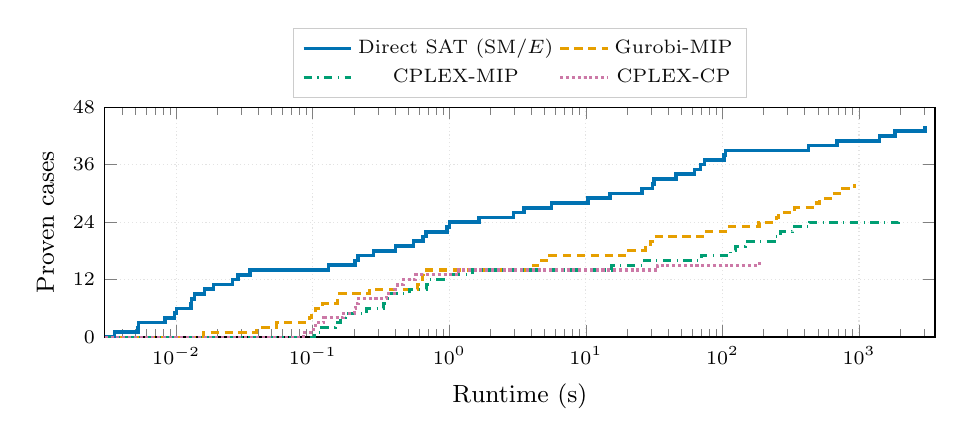
\begin{tikzpicture}
\begin{axis}[width=\linewidth,height=45mm,xmode=log,xmin=0.003,xmax=3600,ymin=0,ymax=48,ytick={0,12,24,36,48},xlabel={Runtime (s)},ylabel={Proven cases},grid=major,grid style={gray!22,densely dotted},legend style={font=\scriptsize,at={(0.5,1.04)},anchor=south,legend columns=2,draw=gray!40,fill=white,fill opacity=0.95},tick label style={font=\scriptsize},label style={font=\small}]
\addplot[const plot,no marks,color=PlotBlue,solid,line width=1.3pt] coordinates {(0.003,0) (0.003541470,1) (0.005247116,2) (0.005295753,3) (0.008251190,4) (0.009734154,5) (0.010025740,6) (0.012866020,7) (0.012958288,8) (0.013652802,9) (0.016139984,10) (0.018746376,11) (0.025910139,12) (0.028381348,13) (0.034771204,14) (0.130478382,15) (0.204934835,16) (0.214081764,17) (0.278077841,18) (0.403787374,19) (0.546904325,20) (0.643606663,21) (0.673460960,22) (0.963696957,23) (1.005735874,24) (1.652459383,25) (2.954896927,26) (3.520453930,27) (5.610790014,28) (10.350619320,29) (14.979071380,30) (25.892252450,31) (30.701663730,32) (31.533023600,33) (45.685124640,34) (62.390542270,35) (69.248304370,36) (73.714394090,37) (102.675891400,38) (105.555170500,39) (427.714209100,40) (692.269913900,41) (1415.457757000,42) (1829.345566000,43) (3046.984778000,44)};
\addlegendentry{Direct SAT (SM/$E$)}
\addplot[const plot,no marks,color=PlotOrange,densely dashed,line width=1.1pt] coordinates {(0.003,0) (0.015736103,1) (0.038957596,2) (0.054211378,3) (0.094443798,4) (0.098404884,5) (0.104360580,6) (0.117602825,7) (0.152279139,8) (0.157175779,9) (0.260886192,10) (0.588612795,11) (0.619363069,12) (0.637070417,13) (0.646924496,14) (4.112289906,15) (4.747301102,16) (5.394608736,17) (19.196970460,18) (27.183960200,19) (29.504277940,20) (31.556227680,21) (76.154961110,22) (105.969540800,23) (185.230606300,24) (248.316510400,25) (258.247517600,26) (338.200370300,27) (456.894193200,28) (514.850428300,29) (637.906011300,30) (762.625196500,31) (930.133920000,32)};
\addlegendentry{Gurobi-MIP}
\addplot[const plot,no marks,color=PlotGreen,dashdotted,line width=1.1pt] coordinates {(0.003,0) (0.103470325,1) (0.113736629,2) (0.145992041,3) (0.160179615,4) (0.174883127,5) (0.249468327,6) (0.331637383,7) (0.336660147,8) (0.371800423,9) (0.509796143,10) (0.684638023,11) (0.715104818,12) (0.908212662,13) (1.468562365,14) (15.349610570,15) (26.812348370,16) (70.230240350,17) (115.213775600,18) (125.066116800,19) (146.385148800,20) (239.075233700,21) (267.683440700,22) (325.308251400,23) (435.926925400,24) (1953.797598000,25)};
\addlegendentry{CPLEX-MIP}
\addplot[const plot,no marks,color=PlotPurple,densely dotted,line width=1.1pt] coordinates {(0.003,0) (0.085296631,1) (0.101630449,2) (0.104367733,3) (0.120749712,4) (0.169259787,5) (0.202065468,6) (0.206754208,7) (0.216585875,8) (0.344884157,9) (0.394920349,10) (0.418884277,11) (0.458345175,12) (0.567824841,13) (1.174881220,14) (33.635968920,15) (185.564700400,16)};
\addlegendentry{CPLEX-CP}
\end{axis}
\end{tikzpicture}
\par\smallskip\footnotesize (a) $Q^{\mathrm{top}}_{\max}$
\end{minipage}
\hfill
\begin{minipage}{0.49\textwidth}
\centering
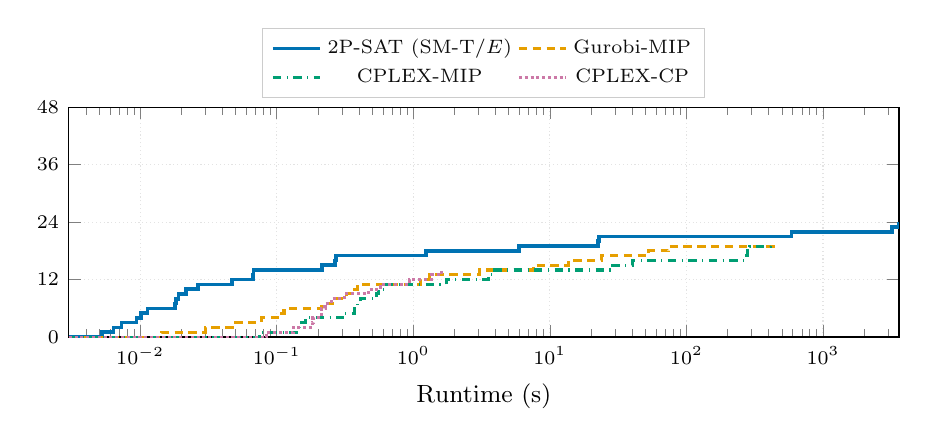
\begin{tikzpicture}
\begin{axis}[width=\linewidth,height=45mm,xmode=log,xmin=0.003,xmax=3600,ymin=0,ymax=48,ytick={0,12,24,36,48},xlabel={Runtime (s)},grid=major,grid style={gray!22,densely dotted},legend style={font=\scriptsize,at={(0.5,1.04)},anchor=south,legend columns=2,draw=gray!40,fill=white,fill opacity=0.95},tick label style={font=\scriptsize},label style={font=\small}]
\addplot[const plot,no marks,color=PlotBlue,solid,line width=1.3pt] coordinates {(0.003,0) (0.005237341,1) (0.006369829,2) (0.007310152,3) (0.009406328,4) (0.010154724,5) (0.011291504,6) (0.018010616,7) (0.018234015,8) (0.019078970,9) (0.021774769,10) (0.026400328,11) (0.046944141,12) (0.066911459,13) (0.067498446,14) (0.213874578,15) (0.268489361,16) (0.272375822,17) (1.245343924,18) (5.948643684,19) (22.627681020,20) (22.932389020,21) (586.137917000,22) (3200.426179000,23) (3586.001296000,24)};
\addlegendentry{2P-SAT (SM-T/$E$)}
\addplot[const plot,no marks,color=PlotOrange,densely dashed,line width=1.1pt] coordinates {(0.003,0) (0.014233112,1) (0.029942036,2) (0.049777985,3) (0.077031136,4) (0.108666658,5) (0.113059759,6) (0.213433027,7) (0.263217449,8) (0.323802948,9) (0.370296955,10) (0.388314009,11) (1.121779442,12) (1.308657169,13) (3.058547735,14) (7.559943438,15) (13.677929160,16) (23.913820980,17) (52.798798320,18) (74.101635220,19) (443.977200000,20)};
\addlegendentry{Gurobi-MIP}
\addplot[const plot,no marks,color=PlotGreen,dashdotted,line width=1.1pt] coordinates {(0.003,0) (0.074887753,1) (0.145617247,2) (0.147617817,3) (0.161184788,4) (0.302835226,5) (0.374069214,6) (0.389798164,7) (0.411795378,8) (0.539725065,9) (0.552820683,10) (0.633949518,11) (1.739472628,12) (3.550043344,13) (3.839728355,14) (27.962858680,15) (40.030714270,16) (274.104711100,17) (280.538741800,18) (290.674826600,19) (414.209457200,20)};
\addlegendentry{CPLEX-MIP}
\addplot[const plot,no marks,color=PlotPurple,densely dotted,line width=1.1pt] coordinates {(0.003,0) (0.084149361,1) (0.132140398,2) (0.182720661,3) (0.184361219,4) (0.211303949,5) (0.212219954,6) (0.225722313,7) (0.250324011,8) (0.311642885,9) (0.468177557,10) (0.575646639,11) (0.937197447,12) (1.363550663,13) (1.621778727,14)};
\addlegendentry{CPLEX-CP}
\end{axis}
\end{tikzpicture}
\par\smallskip\footnotesize (b) $Q^{\mathrm{avg}}_{\max}$
\end{minipage}
\caption{Cumulative number of cases solved to proven optimality within the 3,600-second time limit. The top-$m$-based panel uses Direct SAT (SM/$E$), whereas the average-based panel uses 2P-SAT (SM-T/$E$). Only runs returning \textsc{optimal} contribute; staircase height gives the number of cases proved by the corresponding wall-clock time. Both panels use the same axes.}
\label{fig:cactus}
\end{figure}

\FloatBarrier
\subsection{Descriptive analysis of solving difficulty}

Table~\ref{tab:hardness-strata} groups the 72 cases by whether the selected SAT configuration proves optimality within 3,600 seconds. The number of tasks per station has no clear monotone pattern. Direct precedence density gives the clearest separation: all cases with density above 0.20 are proved under both limits, whereas only 16 of the 44 cases with density at most 0.10 are proved under the top-$m$-based limit, and none of those 44 are proved under the average-based limit. The energy lower-bound ratio shows a similar pattern. Under the top-$m$-based limit, only 1 of 12 cases is proved when $\rho_E>1.25$; under the average-based limit, 13 of 61 such cases are proved.

Proof coverage under graph-balanced weighting reaches \GraphBalancedTopSATProofPct\% and \GraphBalancedAVGSATProofPct\% for $Q_{\max}^{\mathrm{top}}$ and $Q_{\max}^{\mathrm{avg}}$, respectively, compared with \CaseWeightedTopSATProofPct\% and \CaseWeightedAVGSATProofPct\% under standard case-level averaging.

\begin{table}[t!]
\centering
\caption{Cases solved to proven optimality by the selected SAT configuration, grouped by instance characteristics. Entries are proved / total.}
\label{tab:hardness-strata}
\small
\renewcommand{\arraystretch}{1.15}
\setlength{\tabcolsep}{28pt}
\begin{tabular}{@{} l c c @{}}
\toprule
Instance stratum & $Q^{\mathrm{top}}_{\max}$ & $Q^{\mathrm{avg}}_{\max}$ \\
\midrule
\multicolumn{3}{@{}l}{\textit{Tasks per station ($n/m$)}} \\
\addlinespace[2pt]
\quad $n/m\leq2$ & 8 / 10 & 7 / 10 \\
\quad $2<n/m\leq4$ & 23 / 48 & 11 / 48 \\
\quad $n/m>4$ & 13 / 14 & 6 / 14 \\
\addlinespace[4pt]
\multicolumn{3}{@{}l}{\textit{Direct precedence density ($d_E$)}} \\
\addlinespace[2pt]
\quad $d_E\leq0.10$ & 16 / 44 & 0 / 44 \\
\quad $0.10<d_E\leq0.20$ & 11 / 11 & 7 / 11 \\
\quad $d_E>0.20$ & 17 / 17 & 17 / 17 \\
\addlinespace[4pt]
\multicolumn{3}{@{}l}{\textit{Normalized energy lower-bound ratio ($\rho_E$)}} \\
\addlinespace[2pt]
\quad $\rho_E<1$ & 14 / 14 & 1 / 1 \\
\quad $1\leq\rho_E\leq1.25$ & 29 / 46 & 10 / 10 \\
\quad $\rho_E>1.25$ & 1 / 12 & 13 / 61 \\
\bottomrule
\end{tabular}
\end{table}

\FloatBarrier
\subsection{Discussion and limitations}

RQ1 confirms, in the SALBP setting, the mechanism identified in peak-constrained flow shop and job shop research \citep{Fang2013Flow,Carlucci2021A}: a tighter instantaneous power limit restricts concurrency and lengthens the production cycle. The average-based threshold is uniformly tighter and produces substantially larger cycle time increases. The relationship remains instance-dependent, however: cases with similar normalized threshold tightness can exhibit different cycle time penalties because station assignment, precedence structure, task duration, and power demand interact.

RQ2 and RQ3 show that search strategy and encoding influence different aspects of the exact solution process. SM reduces the clause count by approximately one third relative to the Prior CSE baseline; SM-T provides a smaller additional reduction whose computational benefit is encoding- and regime-dependent. The sparse augmentation $E^+$ increases the clause count by fewer than 1.2\% and yields the largest gains under the harder average-based limit. Phase I improves proof coverage with SM-T under the average-based limit but not under the top-$m$-based limit, supporting power-limit-specific rather than universal configuration selection.

RQ4 demonstrates that the selected SAT configurations outperform the commercial comparators on both proof coverage and solution quality. The geometric-mean speedup ratios reach an order of magnitude or more under $Q_{\max}^{\mathrm{top}}$ (Table~\ref{tab:solver-paired}). These ratios reflect deployment-level differences\textemdash{}CaDiCaL runs on a single thread while the commercial solvers use up to eight\textemdash{}rather than per-core algorithmic performance.

The present study is scoped to fixed power demands, integer task durations, constant within-task power, a fixed workstation count, and discrete time. The graph-balanced sensitivity results confirm consistent trends across both weighting schemes. Measured and time-varying power profiles, alternative demand distributions, variable workstation counts, and continuous-time extensions remain directions for future work.

\section{Conclusion}

This study introduces exact cycle time minimization for the simple assembly line balancing problem under a prescribed peak power limit. The SAT formulation combines a compact fixed-horizon encoding with a power-aware analytical lower bound, a guaranteed sequential upper bound, and incremental CDCL incumbent improvement. The Two-phase variant prepends a conflict-limited feasibility search before the incumbent improvement and optimality proof phase.

Three main findings emerge. First, both power-limit constructions increase cycle time relative to the uncapped optimum; the average-based threshold produces substantially larger increases. Second, the SM encoding provides the principal reduction in formula size relative to the Prior CSE baseline, while SM-T and $E^+$ offer complementary but smaller gains. Third, the preferred configuration depends on the power-limit regime: D-SM/$E$ performs best under $Q_{\max}^{\mathrm{top}}$, and 2P-SM-T/$E$ under $Q_{\max}^{\mathrm{avg}}$.

Future work may extend the model to measured and time-varying power profiles, mixed-model and continuous-time settings, variable workstation counts, and stronger analytical lower bounds.

\section*{Acknowledgements}

The authors thank the maintainers of the SALBP benchmark instances and acknowledge the peak-power line-balancing studies that motivated this work.

\section*{Disclosure statement}

The authors report there are no competing interests to declare.

\section*{Funding}

The authors received no specific grant from any funding agency in the public, commercial or not-for-profit sectors for this research.

\section*{Data availability statement}

The benchmark data, task power-demand vectors, source code, and result tables are available from the corresponding author upon reasonable request.

\bibliographystyle{tfcad}
\bibliography{refs}

\end{document}
